\documentclass{article}




\usepackage{fullpage}
\usepackage{nopageno}
\usepackage{amsmath}
\usepackage{amsfonts}
\usepackage{graphicx}
\usepackage{framed}
\usepackage{algorithmic}
\usepackage{xcolor}

\definecolor{dark_red}{rgb}{0.5,0.0,0.0}
\definecolor{dark_green}{rgb}{0.0,0.5,0.0}
\definecolor{dark_blue}{rgb}{0.0,0.0,0.5}
\definecolor{blue}{rgb}{0.0,0.0,1.0}

\newcommand{\dr}[1]{\textcolor{dark_red}{#1}}
\newcommand{\dg}[1]{\textcolor{dark_green}{#1}}
\newcommand{\db}[1]{\textcolor{dark_blue}{#1}}
\newcommand{\blue}[1]{\textcolor{blue}{#1}}


\usepackage{fancyhdr}
%\setlength{\footheight}{15.2pt}
\pagestyle{fancy}
\fancyhead[C]{Wentworth Institute of Technology, MATH2025}
\fancyfoot[C]{Author: Shawn Eastwood}
\renewcommand{\headsep}{25pt}
\renewcommand{\headrulewidth}{1pt}
\renewcommand{\footrulewidth}{1pt}



\begin{document}

\section*{Position vectors}

\begin{tabular}{cc}
\parbox{0.5\textwidth}{
Given an arbitrary point \((x, y, z)\) in Cartesian coordinates, the {\bf position vector} \(\mathbf{q} = \begin{bmatrix} x \\ y \\ z \end{bmatrix}\) will be synonymous with the point \((x, y, z)\), and the two notations will be interchangeable. The position vector \(\mathbf{q} = \begin{bmatrix} x \\ y \\ z \end{bmatrix}\) is the displacement vector from the {\bf origin} to the point \((x,y,z)\). Given two points \(\mathbf{q}_A = \begin{bmatrix} x_A \\ y_A \\ z_A \end{bmatrix}\) and \(\mathbf{q}_B = \begin{bmatrix} x_B \\ y_B \\ z_B \end{bmatrix}\), the vector difference \(\mathbf{q}_B - \mathbf{q}_A = \begin{bmatrix} x_B - x_A \\ y_B - y_A \\ z_B - z_A \end{bmatrix}\) is the displacement from point \(\mathbf{q}_A\) to \(\mathbf{q}_B\). 
} & \parbox{0.5\textwidth}{
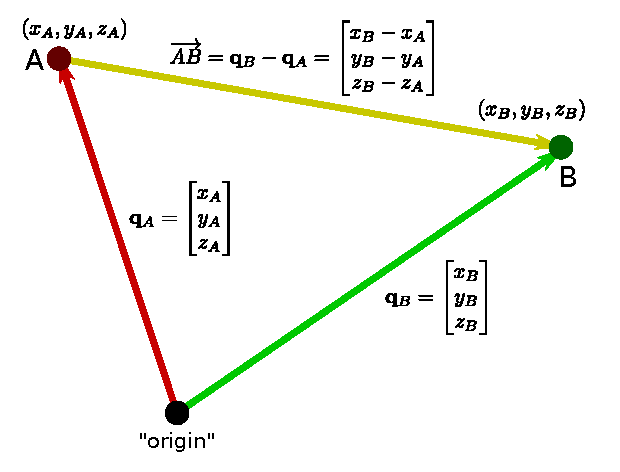
\includegraphics[width = 0.5\textwidth]{position_vectors_and_displacements}
}
\end{tabular}

\vspace{5mm}




\section*{Vector and parametric equations}

Before now, curves and surfaces are quantified by listing one or multiple equations that all points on the curve or surface must satisfy. Now, additional variables, referred to as {\bf parameters}, will be used to quantify curves and surfaces. With a parametric curve or surface, each coordinate is an explicit function of the parameter variables. Each assignment to the parameter values, from the domain of valid parameter values, will generate a point that lies on the curve or surface. 

When a set of equations is listed, a point can be arbitrarily chosen, and then determined as to whether the point lies on the curve/surface or not. This traditional approach of describing a curve or surface by listing equations that all points must satisfy is referred to as an {\bf implicit} description. 

When parametric equations are used, points can be generated directly by setting the parameter values as opposed to choosing a point and then ``testing" whether the point is on the curve or not.

Two ``forms" of parametric equations will be addressed:
\begin{itemize}
\item A {\bf vector equation} is a parametric equation, where the position vector of the generated point is expressed as an expression involving vectors and the parameters. Vector equations have the following form:
\[\mathbf{q}(t) = \;\; <\textnormal{expression involving vectors and the parameter \(t\)}>\]
\item A basic set of parametric equations for a set of points in space has an independent expression for each coordinate. The parameters are shared between the expressions however. Parametric equations have the following form:
\[\left\{\begin{array}{c} 
x(t) = \;\; <\textnormal{expression involving the parameter \(t\)}> \\
y(t) = \;\; <\textnormal{expression involving the parameter \(t\)}> \\
z(t) = \;\; <\textnormal{expression involving the parameter \(t\)}> \\
\end{array}\right.\]
\end{itemize}
Note that there may in fact be more parameters than \(t\). 

\textbf{Example:}

\begin{itemize}
\item Consider the parametric equations:
\[\left\{\begin{array}{l} 
x(t) = 3 - 5t \\ 
y(t) = 2 + 2t \\ 
z(t) = 7 - 3t
\end{array}\right.\]
These parametric equations describe a curve in 3D space. Various values of \(t\) will generate various points on the curve:
\begin{align*}
t = -3 \implies & (x,y,z) = (18, -4, 16) \\
t = -1 \implies & (x,y,z) = (8, 0, 10) \\
t = 0 \implies & (x,y,z) = (3, 2, 7) \\
t = 2 \implies & (x,y,z) = (-7, 6, 1)
\end{align*}
The parametric equations for a curve are {\bf not unique}. Consider the parametric equations:
\[\left\{\begin{array}{l}
x(t) = -2 + 10t \\ 
y(t) = 4 - 4t \\ 
z(t) = 4 + 6t
\end{array}\right.\]
This curve is equivalent to the previous curve, despite the fact that the parametric equations are different. The following values of \(t\) will generate the same points:
\begin{align*}
t = 2 \implies & (x,y,z) = (18, -4, 16) \\
t = 1 \implies & (x,y,z) = (8, 0, 10) \\
t = \frac{1}{2} \implies & (x,y,z) = (3, 2, 7) \\
t = -\frac{1}{2} \implies & (x,y,z) = (-7, 6, 1)
\end{align*}
The change is that the same points are now being generated by different values of \(t\).
\end{itemize}



In summary, 
\begin{itemize}
%%%%%%%%%%%%%%%%%%%%%%%%%%%%%%%%
\item An {\bf explicit} description of curve or surface involves a function(s) that can compute any point on the curve/surface given an appropriate choice of parameter values. For curves, 1 parameter is needed:
\[\mathbf{q}(t) = \begin{bmatrix} <\textnormal{expression involving the parameter \(t\)}> \\ <\textnormal{expression involving the parameter \(t\)}> \\ <\textnormal{expression involving the parameter \(t\)}> \end{bmatrix}\] 
For surfaces, 2 parameters are needed:
\[\mathbf{q}(t_1, t_2) = \begin{bmatrix} <\textnormal{expression involving the parameters \(t_1\) and \(t_2\)}> \\ <\textnormal{expression involving the parameters \(t_1\) and \(t_2\)}> \\ <\textnormal{expression involving the parameters \(t_1\) and \(t_2\)}> \end{bmatrix}\] 
From the explicit/parametric description of a curve/surface, it is {\bf easy} to generate points that lie on the curve/surface by choosing various values for the parameters. Given an arbitrary point however, it is {\bf not easy} to determine whether or not this point lies on the curve/surface.
%%%%%%%%%%%%%%%%%%%%%%%%%%%%%%%%
\item An {\bf implicit} description of curve or surface involves equations that must all be satisfied for a point \(\mathbf{q} = \begin{bmatrix} x \\ y \\ z \end{bmatrix}\) to lie on the curve/surface. For curves, 2 equations are needed:
\[\left\{\begin{array}{c} <\textnormal{equation involving \(x\), \(y\), and \(z\)}> \\ <\textnormal{equation involving \(x\), \(y\), and \(z\)}> \end{array}\right.\]  
For surfaces, 1 equation is needed:
\[\left\{\begin{array}{c} <\textnormal{equation involving \(x\), \(y\), and \(z\)}> \end{array}\right.\]
From the implicit description of a curve/surface, it is {\bf easy} to determine whether or not a given point lies on the curve/surface by checking if all equations are satisfied. It is {\bf not easy} however to generate points that lie on the curve/surface. 
\end{itemize}

\textbf{Example:}

\begin{itemize}
\item Consider the parametric equations:
\[\left\{\begin{array}{l}
x(t) = 2 + 2\cos(t) \\ 
y(t) = -1 + \sin(t) \\ 
z(t) = \sin(t)
\end{array}\right.\]
As well as the implicit equations:
\[\left\{\begin{array}{c}
x^2 + 4y^2 - 4x + 8y = -4 \\
z = y + 1
\end{array}\right.\]
Both of these systems describe the same curve. 

If arbitrary points on the curve are what is required, then arbitrary values of \(t\) can be substituted into the parametric equations to generate arbitrary points:
\begin{align*}
t = \pi/4 \implies & (x,y,z) = \left(2 + \sqrt{2}, -1 + \frac{1}{\sqrt{2}}, \frac{1}{\sqrt{2}}\right) \\   
t = 3\pi/4 \implies & (x,y,z) = \left(2 - \sqrt{2}, -1 + \frac{1}{\sqrt{2}}, \frac{1}{\sqrt{2}}\right)
\end{align*}

If the status of whether or not a point lies on the curve is what is required, then the implicit equations, if all satisfied, determines that the point lies on the curve.  
\begin{itemize}
\item[*] Given the point \((x, y, z) = (4, -1, 0)\), the two sides of the first equation evaluate to: 
\begin{align*}
\text{LHS} = & x^2 + 4y^2 - 4x + 8y = 4^2 + 4(-1)^2 - 4(4) + 8(-1) = 16 + 4 - 16 - 8 = -4 \\ 
\text{RHS} = & -4
\end{align*} 
so the first equation is satisfied. The two sides of the second equation evaluate to:
\begin{align*}
\text{LHS} = & z = 0 \\ 
\text{RHS} = & y + 1 = 0
\end{align*}
so the second equation is satisfied. Both equations are satisfied so \((4, -1, 0)\) lies on the curve. 
\end{itemize}
\item[*] Given the point \((x, y, z) = (2, 0, 0)\), the two sides of the first equation evaluate to: 
\begin{align*}
\text{LHS} = & x^2 + 4y^2 - 4x + 8y = 2^2 + 4(0)^2 - 4(2) + 8(0) = 4 + 0 - 8 + 0 = -4 \\ 
\text{RHS} = & -4
\end{align*} 
so the first equation is satisfied. The two sides of the second equation evaluate to:
\begin{align*}
\text{LHS} = & z = 0 \\ 
\text{RHS} = & y + 1 = 1
\end{align*}
so the second equation is not satisfied. Since not both of the equations are satisfied, point \((2, 0, 0)\) does not lie on the curve. 
\end{itemize}




\section*{The equations of lines}

\subsection*{Parametric equations for lines}

\begin{tabular}{cc}
\parbox{0.5\textwidth}{
Consider an arbitrary point with position vector \(\mathbf{q}_0 = \begin{bmatrix} x_0 \\ y_0 \\ z_0 \end{bmatrix}\) and a nonzero direction vector \(\mathbf{v} = \begin{bmatrix} v_x \\ v_y \\ v_z \end{bmatrix}\). Let \(L\) denote the line that passes through \(\mathbf{q}_0\) and is parallel to vector \(\mathbf{v}\). Adding any multiple of \(\mathbf{v}\) to \(\mathbf{q}_0\) will generate a point from \(L\), and for every point \(\mathbf{q}\) that belongs to \(L\), the displacement \(\mathbf{q} - \mathbf{q}_0\) is some multiple of \(\mathbf{v}\). One possible vector equation of the line is:
\[\mathbf{q}(t) = \mathbf{q}_0 + \mathbf{v}t\]
In this case, \(t = 0\) generates the point \(\mathbf{q}_0\). 
} & \parbox{0.5\textwidth}{
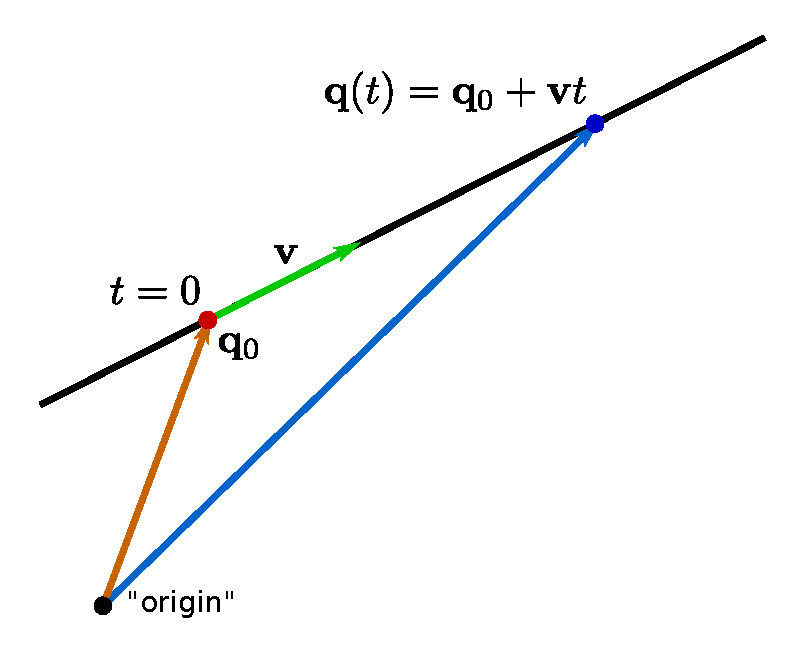
\includegraphics[width = 0.5\textwidth]{vector_equation_line}
}
\end{tabular}
The parametric equations themselves are:
\begin{align*}
& \begin{bmatrix} x(t) \\ y(t) \\ z(t) \end{bmatrix} = \begin{bmatrix} x_0 \\ y_0 \\ z_0 \end{bmatrix} + \begin{bmatrix} v_x \\ v_y \\ v_z \end{bmatrix}t = \begin{bmatrix} x_0 + v_x t \\ y_0 + v_y t \\ z_0 + v_z t \end{bmatrix} 
\iff \left\{\begin{array}{c} x(t) = x_0 + v_x t \\ y(t) = y_0 + v_y t \\ z(t) = z_0 + v_z t \end{array}\right.
\end{align*}

\begin{tabular}{cc}
\parbox{0.4\textwidth}{
It should be noted that parametric equations are not unique. The same curve/surface may have different parametric equations where the same value of \(t\) will generate different points. As an example, consider the line \(L\) that passes through a point with position vector \(\mathbf{q}_0\) and is parallel to vector \(\mathbf{v}\). This, as discussed above, yields the vector equation \(\mathbf{q}(t) = \mathbf{q}_0 + \mathbf{v}t\). Line \(L\) also passes through the point with position vector \(\mathbf{q}_0 + 3\mathbf{v}\), and is parallel to the vector \(-2\mathbf{v}\). This yields the vector equation \(\mathbf{q}(t) = (\mathbf{q}_0 + 3\mathbf{v}) - 2\mathbf{v}t\) which yields a different set of parametric equations.
} & \parbox{0.6\textwidth}{
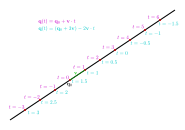
\includegraphics[width = 0.6\textwidth]{multiple_parameterizations}
}
\end{tabular}

\begin{tabular}{cc}
\parbox{0.5\textwidth}{
The line {\bf segment} from point \(\mathbf{q}_0 = \begin{bmatrix} x_0 \\ y_ 0 \\ z_0 \end{bmatrix}\) to point \(\mathbf{q}_1 = \begin{bmatrix} x_1 \\ y_1 \\ z_1 \end{bmatrix}\) has the vector equation:   
\[\mathbf{q}(t) = \mathbf{q}_0 + (\mathbf{q}_1 - \mathbf{q}_0)t  = (1 - t)\mathbf{q}_0 + t \mathbf{q}_1\]
The parameter \(t\) is confined to the interval \([0, 1]\). When \(t = 0\), \(\mathbf{q}(0) = \mathbf{q}_0\). When \(t = 1\), \(\mathbf{q}(1) = \mathbf{q}_1\). 
} & \parbox{0.5\textwidth}{
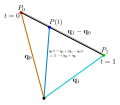
\includegraphics[width = 0.5\textwidth]{vector_equation_line_segment}
}
\end{tabular}
The parametric equations themselves are:
\[\left\{\begin{array}{c} x(t) = x_0 + (x_1 - x_0)t = (1 - t)x_0 + t x_1 \\ y(t) = y_0 + (y_1 - y_0)t = (1 - t)y_0 + t y_1 \\ z(t) = z_0 + (z_1 - z_0)t = (1 - t)z_0 + t z_1\end{array}\right. \quad (0 \leq t \leq 1)\]
The parameter \(t\) is confined to the interval \([0, 1]\).

\textbf{Examples:}
\begin{itemize}
%%%%%%%%%%%%%%%%%%%%%%%%%%%
\item Given the points \(X(7, 1, -5)\) and \(Y(2, -3, -6)\), the line that passes through \(X\) and \(Y\) must be parallel to \(\overrightarrow{XY} = \begin{bmatrix} 2 - 7 \\ (-3) - 1 \\ (-6) - (-5) \end{bmatrix} = \begin{bmatrix} -5 \\ -4 \\ -1 \end{bmatrix}\). One possible vector equation is:
\[\mathbf{q}(t) = \begin{bmatrix} 7 \\ 1 \\ -5 \end{bmatrix} + \begin{bmatrix} -5 \\ -4 \\ -1 \end{bmatrix}t\] 
The corresponding set of parametric equations is: 
\[\left\{\begin{array}{c} x(t) = 7 - 5t \\ y(t) = 1 - 4t \\ z(t) = -5 - t \end{array}\right.\]
Another set of parametric equations can be derived by observing that the line passes through the point where \(t = 2\): \(\mathbf{q}(2) = \begin{bmatrix} -3 \\ -7 \\ -7 \end{bmatrix}\), and is parallel to the vector \(-3\overrightarrow{XY} = \begin{bmatrix} 15 \\ 12 \\ 3 \end{bmatrix}\) Another vector equation {\bf of the same line} is: 
\[\mathbf{q}(t) = \begin{bmatrix} -3 \\ -7 \\ -7 \end{bmatrix} + \begin{bmatrix} 15 \\ 12 \\ 3 \end{bmatrix}t\] 
The corresponding set of parametric equations is: 
\[\left\{\begin{array}{c} x(t) = -3 + 15t \\ y(t) = -7 + 12t \\ z(t) = -7 + 3t \end{array}\right.\]
%%%%%%%%%%%%%%%%%%%%%%%%%%%
\item Given the points \(B(8, 1, -2)\) and \(A(1, -7, 3)\), the line that passes through \(B\) and \(A\) must be parallel to \(\overrightarrow{BA} = \begin{bmatrix} 1 - 8 \\ (-7) - 1 \\ 3 - (-2) \end{bmatrix} = \begin{bmatrix} -7 \\ -8 \\ 5 \end{bmatrix}\). One possible vector equation is:
\[\mathbf{q}(t) = \begin{bmatrix} 8 \\ 1 \\ -2 \end{bmatrix} + \begin{bmatrix} -7 \\ -8 \\ 5 \end{bmatrix}t\]
The corresponding set of parametric equations is: 
\[\left\{\begin{array}{c} x(t) = 8 - 7t \\ y(t) = 1 - 8t \\ z(t) = -2 + 5t \end{array}\right.\]
%%%%%%%%%%%%%%%%%%%%%%%%%%%
\item Given the points \(M(0, -7, 2)\) and \(C(4, 5, 0)\), the line that passes through \(M\) and \(C\) must be parallel to \(\overrightarrow{MC} = \begin{bmatrix} 4 - 0 \\ 5 - (-7) \\ 0 - 2 \end{bmatrix} = \begin{bmatrix} 4 \\ 12 \\ -2 \end{bmatrix}\). One possible vector equation is:
\[\mathbf{q}(t) = \begin{bmatrix} 0 \\ -7 \\ 2 \end{bmatrix} + \begin{bmatrix} 4 \\ 12 \\ -2 \end{bmatrix}t\]
The corresponding set of parametric equations is:
\[\left\{\begin{array}{c} x(t) = 4t \\ y(t) = -7 + 12t \\ z(t) = 2 - 2t \end{array}\right.\]
\end{itemize}



\vspace{5mm}

\subsection*{Implicit equations for lines}

Any line in 3 dimensions can be implicitly described by listing \(2\) equations:

\[\left\{\begin{array}{c}
a_1 x + b_1 y + c_1 z = d_1 \\ 
a_2 x + b_2 y + c_2 z = d_2 
\end{array}\right.\]

Often, what is desired is not simply 2 equations, but equations of the form:
\[f_x x + g_x = f_y y + g_y = f_z z + g_z\]
This is the equivalence of \(3\) quantities, where each quantity is a linear function of exactly \(1\) variable. These equations are also called the {\bf symmetric} equation of a line. 

Given the parametric equations:
\[\left\{\begin{array}{c} x(t) = x_0 + v_x t \\ y(t) = y_0 + v_y t \\ z(t) = z_0 + v_z t \end{array}\right.\]
which describe a line, how can an implicit set of equations be derived? Let \((x, y, z)\) be an arbitrary point. \((x, y, z)\) lies on the line if and only if there exists some value of \(t\) such that \(x = x_0 + v_x t\); \(y = y_0 + v_y t\); and \(z = z_0 + v_z t\). Solving each equation for \(t\) gives respectively: \(t = \frac{x - x_0}{v_x}\); \(t = \frac{y - y_0}{v_y}\); and \(t = \frac{z - z_0}{v_z}\). All of these values of \(t\) must be equivalent, which means that for point \((x, y, z)\) to lie on the line,
\[\frac{x - x_0}{v_x} = \frac{y - y_0}{v_y} = \frac{z - z_0}{v_z}\]    
these are the symmetric equations of the line.  

What if one of \(v_x\), \(v_y\), or \(v_z\) is actually \(0\)? If for example \(v_x = 0\) but \(v_y\) and \(v_z\) are nonzero, then the symmetric equations are instead:
\[\left\{\begin{array}{c}
x = x_0 \\ 
\frac{y - y_0}{v_y} = \frac{z - z_0}{v_z}
\end{array}\right.\]

Given the two equations,
\[\left\{\begin{array}{c}
a_1 x + b_1 y + c_1 z = d_1 \\ 
a_2 x + b_2 y + c_2 z = d_2 
\end{array}\right.\]
how can parametric equations for the line be derived? By solving the system, two of the coordinates are a function of the remaining coordinate. By setting the remaining coordinate equal to \(t\), then the other coordinates are functions of \(t\) and then all \(3\) coordinates are functions of \(t\). From the parametric equation, symmetric equations can be derived. 

\textbf{Examples:}
\begin{itemize}
%%%%%%%%%%%%%%%%%%%%%%%%%%%%%%%%%%%%%%%%%%%%%%%%%%%%
\item Consider the line \(L\) with the parametric equations: 
\[\left\{\begin{array}{c}
x(t) = 2 - 4t \\ 
y(t) = 5 - \frac{1}{2}t \\ 
z(t) = 1 + \frac{1}{3}t
\end{array}\right.
\quad\quad\text{the vector equation is:}\quad\quad
\mathbf{q}(t) = \begin{bmatrix} 2 \\ 5 \\ 1 \end{bmatrix} + \begin{bmatrix} -4 \\ -\frac{1}{2} \\ \frac{1}{3} \end{bmatrix}t\]
Let \((x, y, z)\) denote an arbitrary point. Solving for \(t\) from each of the parametric equations gives: \(t = \frac{x - 2}{-4} = \frac{2 - x}{4}\); \(t = \frac{y - 5}{-1/2} = 10 - 2y\); and \(t = \frac{z - 1}{1/3} = 3z - 3\). These 3 values of \(t\) must all be equal so:
\[\frac{2 - x}{4} = 10 - 2y = 3z - 3\]
are the symmetric equations for \(L\).
%%%%%%%%%%%%%%%%%%%%%%%%%%%%%%%%%%%%%%%%%%%%%%%%%%%%
\item Consider the line \(L\) with the parametric equations: 
\[\left\{\begin{array}{c}
x(t) = -3 \\ 
y(t) = \frac{3}{2} - \frac{1}{2}t \\ 
z(t) = 4 - 2t
\end{array}\right.
\quad\quad\text{the vector equation is:}\quad\quad
\mathbf{q}(t) = \begin{bmatrix} -3 \\ \frac{3}{2} \\ 4 \end{bmatrix} + \begin{bmatrix} 0 \\ -\frac{1}{2} \\ -2 \end{bmatrix}t\]
Let \((x, y, z)\) denote an arbitrary point. The first equation simply requires \(x = -3\). Solving for \(t\) from the 2 latter equations gives: \(t = \frac{y - 3/2}{-1/2} = 3 - 2y\); and \(t = \frac{z - 4}{-2} = \frac{4 - z}{2}\). These 2 values of \(t\) must all be equal so:
\[3 - 2y = \frac{4 - z}{2}\]
The equations:
\[\left\{\begin{array}{c}
x = -3 \\ 
3 - 2y = \frac{4 - z}{2}
\end{array}\right.\]
are the symmetric equations for \(L\).
%%%%%%%%%%%%%%%%%%%%%%%%%%%%%%%%%%%%%%%%%%%%%%%%%%%%
\item Consider the line \(L\) with the parametric equations: 
\[\left\{\begin{array}{c}
x(t) = -1 \\ 
y(t) = 4 - t \\ 
z(t) = 3
\end{array}\right.
\quad\quad\text{the vector equation is:}\quad\quad
\mathbf{q}(t) = \begin{bmatrix} -1 \\ 4 \\ 3 \end{bmatrix} + \begin{bmatrix} 0 \\ -1 \\ 0 \end{bmatrix}t\]
There is only 1 value of \(t\) that can be computed from the parametric equations, and since only there is only 1 candidate value for \(t\), no equation can be formed from the expression for \(t\). The two equations that define \(L\) are: 
\[\left\{\begin{array}{c}
x = -1 \\ 
z = 3 
\end{array}\right.\]
%%%%%%%%%%%%%%%%%%%%%%%%%%%%%%%%%%%%%%%%%%%%%%%%%%%%
\item Consider the line \(L\) with the symmetric equations: 
\[3x - 4 = -y + 2 = \frac{1}{3}z - 1\]
The common value of the 3 expressions is \(t\). Solving the 3 equations:
\[\left\{\begin{array}{cc}
3x - 4 = t & \iff x = \frac{t + 4}{3} = \frac{4}{3} + \frac{1}{3}t \\ 
-y + 2 = t & \iff y = \frac{t - 2}{-1} = 2 - t \\ 
\frac{1}{3}z - 1 = t & \iff z = \frac{t + 1}{1/3} = 3 + 3t
\end{array}\right.\]
gives the parametric equations:
\[\left\{\begin{array}{c}
x(t) = \frac{4}{3} + \frac{1}{3}t \\ 
y(t) = 2 - t \\ 
z(t) = 3 + 3t 
\end{array}\right.
\quad\quad\text{the vector equation is:}\quad\quad
\mathbf{q}(t) = \begin{bmatrix} \frac{4}{3} \\ 2 \\ 3 \end{bmatrix} + \begin{bmatrix} \frac{1}{3} \\ -1 \\ 3 \end{bmatrix}t\]
%%%%%%%%%%%%%%%%%%%%%%%%%%%%%%%%%%%%%%%%%%%%%%%%%%%%
\item Consider the line \(L\) which is the set of all \((x,y,z)\) points that satisfy the equations:
\[\left\{\begin{array}{c}
-2x + y + 2z = -2 \\ 
x + 2z = 3
\end{array}\right.\]
Parametric equations for \(L\) are desired. When solving the system, it is important to determine an ``ordering" for the variables. This ordering will determine which variables are solved for as functions of the other variables. Consider for example the ordering \(x, y, z\). Firstly \(z\) will be solved for in the first equation as a function of the other variables \(x\) and \(y\). 
\[-2x + y + 2z = -2 \iff 2z = -2 + 2x - y \iff z = -1 + x - \frac{1}{2}y\]
The expression for \(z\) will then eliminate \(z\) in the second equation. Next \(y\) will be solved for in the second equation as a function of \(x\) alone.
\begin{align*}
& x + 2z = 3 \iff x + 2(-1 + x - \frac{1}{2}y) = 3 \iff x + (-2 + 2x - y) = 3 \iff -y = 5 - 3x \\
& \iff y = -5 + 3x
\end{align*}
The expression for \(y\) can then eliminate \(y\) in the expression for \(z\):
\[z = -1 + x - \frac{1}{2}y = -1 + x + (\frac{5}{2} - \frac{3}{2}x) = \frac{3}{2} - \frac{1}{2}x\]
Now with \(y\) and \(z\) as expressions of \(x\), let \(x = t\). \(x\), \(y\), and \(z\) as functions of \(t\) are:
\[\left\{\begin{array}{c}
x(t) = t \\ 
y(t) = -5 + 3t \\ 
z(t) = \frac{3}{2} - \frac{1}{2}t
\end{array}\right.
\quad\quad\text{the vector equation is:}\quad\quad
\mathbf{q}(t) = \begin{bmatrix} 0 \\ -5 \\ \frac{3}{2} \end{bmatrix} + \begin{bmatrix} 1 \\ 3 \\ -\frac{1}{2} \end{bmatrix}t\]
The symmetric equations are:
\[\frac{x - 0}{1} = \frac{y - (-5)}{3} = \frac{z - 3/2}{-1/2} \iff x = \frac{y + 5}{3} = 3 - 2z\]
%%%%%%%%%%%%%%%%%%%%%%%%%%%%%%%%%%%%%%%%%%%%%%%%%%%%
\item Consider the line \(L\) which is the set of all \((x,y,z)\) points that satisfy the equations:
\[\left\{\begin{array}{c}
5x + 3y + z = 4 \\ 
2x + y - z = 1
\end{array}\right.\]
Parametric equations for \(L\) are desired. When solving the system, it is important to determine an ``ordering" for the variables. This ordering will determine which variables are solved for as functions of the other variables. Consider for example the ordering \(x, y, z\). Firstly \(z\) will be solved for in the first equation as a function of the other variables \(x\) and \(y\). 
\[5x + 3y + z = 4 \iff z = 4 - 5x - 3y\]
The expression for \(z\) will then eliminate \(z\) in the second equation. Next \(y\) will be solved for in the second equation as a function of \(x\) alone.
\begin{align*}
& 2x + y - z = 1 \iff 2x + y - (4 - 5x - 3y) = 1 \iff 2x + y + (-4 + 5x + 3y) = 1 \iff 4y = 5 - 7x \\
& \iff y = \frac{5}{4} - \frac{7}{4}x
\end{align*}
The expression for \(y\) can then eliminate \(y\) in the expression for \(z\):
\[z = 4 - 5x - 3y = 4 - 5x + (-\frac{15}{4} + \frac{21}{4}x) = \frac{1}{4} + \frac{1}{4}x\]
Now with \(y\) and \(z\) as expressions of \(x\), let \(x = t\). \(x\), \(y\), and \(z\) as functions of \(t\) are:
\[\left\{\begin{array}{c}
x(t) = t \\ 
y(t) = \frac{5}{4} - \frac{7}{4}t \\ 
z(t) = \frac{1}{4} + \frac{1}{4}t
\end{array}\right.
\quad\quad\text{the vector equation is:}\quad\quad
\mathbf{q}(t) = \begin{bmatrix} 0 \\ \frac{5}{4} \\ \frac{1}{4} \end{bmatrix} + \begin{bmatrix} 1 \\ -\frac{7}{4} \\ \frac{1}{4} \end{bmatrix}t\]
The symmetric equations are:
\[\frac{x - 0}{1} = \frac{y - 5/4}{-7/4} = \frac{z - 1/4}{1/4} \iff x = \frac{5 - 4y}{7} = 4z - 1\]
%%%%%%%%%%%%%%%%%%%%%%%%%%%%%%%%%%%%%%%%%%%%%%%%%%%%
\item Consider the line \(L\) which is the set of all \((x,y,z)\) points that satisfy the equations:
\[\left\{\begin{array}{c}
2x + y + z = 13 \\ 
-2x + 3y + 3z = 15
\end{array}\right.\]
Parametric equations for \(L\) are desired. When solving the system, it is important to determine an ``ordering" for the variables. This ordering will determine which variables are solved for as functions of the other variables. Consider for example the ordering \(x, y, z\). Firstly \(z\) will be solved for in the first equation as a function of the other variables \(x\) and \(y\). 
\[2x + y + z = 13 \iff z = 13 - 2x - y\]
The expression for \(z\) will then eliminate \(z\) in the second equation. Next \(y\) will be solved for in the second equation as a function of \(x\) alone.
\begin{align*}
& -2x + 3y + 3z = 15 \iff -2x + 3y + 3(13 - 2x - y) = 15 \iff -2x + 3y + (39 - 6x - 3y) = 15 \\
& \iff -8x = -24 \iff x = 3
\end{align*}
The equation gave no information about \(y\), but instead gave a single value for \(x\). The value for \(x\) can then eliminate \(x\) in the expression for \(z\):
\[z = 13 - 2x - y = 13 - 6 - y = 7 - y\]
Now with \(x\) known and \(z\) as an expressions of \(y\), let \(y = t\). \(x\), \(y\), and \(z\) as functions of \(t\) are:
\[\left\{\begin{array}{c}
x(t) = 3 \\ 
y(t) = t \\ 
z(t) = 7 - t
\end{array}\right.
\quad\quad\text{the vector equation is:}\quad\quad
\mathbf{q}(t) = \begin{bmatrix} 3 \\ 0 \\ 7 \end{bmatrix} + \begin{bmatrix} 0 \\ 1 \\ -1 \end{bmatrix}t\]
The symmetric equations are:
\[\left\{\begin{array}{c}
x = 3 \\
\frac{y - 0}{1} = \frac{z - 7}{-1}\end{array}\right. \iff 
\left\{\begin{array}{c}
x = 3 \\
y = 7 - z\end{array}\right.\]
%%%%%%%%%%%%%%%%%%%%%%%%%%%%%%%%%%%%%%%%%%%%%%%%%%%%
\item Consider the line \(L\) which is the set of all \((x,y,z)\) points that satisfy the equations:
\[\left\{\begin{array}{c}
3x - 4y = 7 \\ 
2x - 5y = 0
\end{array}\right.\]
Parametric equations for \(L\) are desired. When solving the system, it is important to determine an ``ordering" for the variables. This ordering will determine which variables are solved for as functions of the other variables. Consider for example the ordering \(x, y, z\). \(z\) appears nowhere in the equations, and cannot be solved for. Instead \(y\) will be solved for in the first equation as a function of the remaining variable \(x\). 
\[3x - 4y = 7 \iff -4y = 7 - 3x \iff y = -\frac{7}{4} + \frac{3}{4}x\]
The expression for \(y\) will then eliminate \(y\) in the second equation. Next \(x\) will be solved for in the second equation.
\begin{align*}
& 2x - 5y = 0 \iff 2x - 5(-\frac{7}{4} + \frac{3}{4}x) = 0 \iff 2x + (\frac{35}{4} - \frac{15}{4}x) = 0 \\
& \iff -\frac{7}{4}x = -\frac{35}{4} \iff x = 5
\end{align*}
The value for \(x\) can then eliminate \(x\) in the expression for \(y\):
\[y = -\frac{7}{4} + \frac{3}{4}x = -\frac{7}{4} + \frac{15}{4} = 2\]
Now with \(x\) and \(y\) known, let \(z = t\). \(x\), \(y\), and \(z\) as functions of \(t\) are:
\[\left\{\begin{array}{c}
x(t) = 5 \\ 
y(t) = 2 \\ 
z(t) = t
\end{array}\right.
\quad\quad\text{the vector equation is:}\quad\quad
\mathbf{q}(t) = \begin{bmatrix} 5 \\ 2 \\ 0 \end{bmatrix} + \begin{bmatrix} 0 \\ 0 \\ 1 \end{bmatrix}t\]
The symmetric equations are:
\[\left\{\begin{array}{c}
x = 5 \\
y = 2 \end{array}\right.\]
\end{itemize}






\section*{The equations of planes}

\subsection*{Parametric equations for planes}

Consider an arbitrary point \(\mathbf{q}_0 = \begin{bmatrix} x_0 \\ y_0 \\ z_0 \end{bmatrix}\) and two nonzero vectors \(\mathbf{v}_1 = \begin{bmatrix} v_{1x} \\ v_{1y} \\ v_{1z} \end{bmatrix}\) and \(\mathbf{v}_2 = \begin{bmatrix} v_{2x} \\ v_{2y} \\ v_{2z} \end{bmatrix}\) that are {\bf not parallel}.
One possible vector equation of the plane that contains point \(\mathbf{q}_0\) and is parallel to \(\mathbf{v}_1\) and \(\mathbf{v}_2\) is:
\begin{align*}
& \mathbf{q}(t_1, t_2) = \mathbf{q}_0 + \mathbf{v}_1 t_1 + \mathbf{v}_2 t_2 
\end{align*}
Note that there are {\bf 2} parameters as opposed to only 1 parameter as is the case for lines.

\begin{tabular}{cc}
\parbox{0.5\textwidth}{
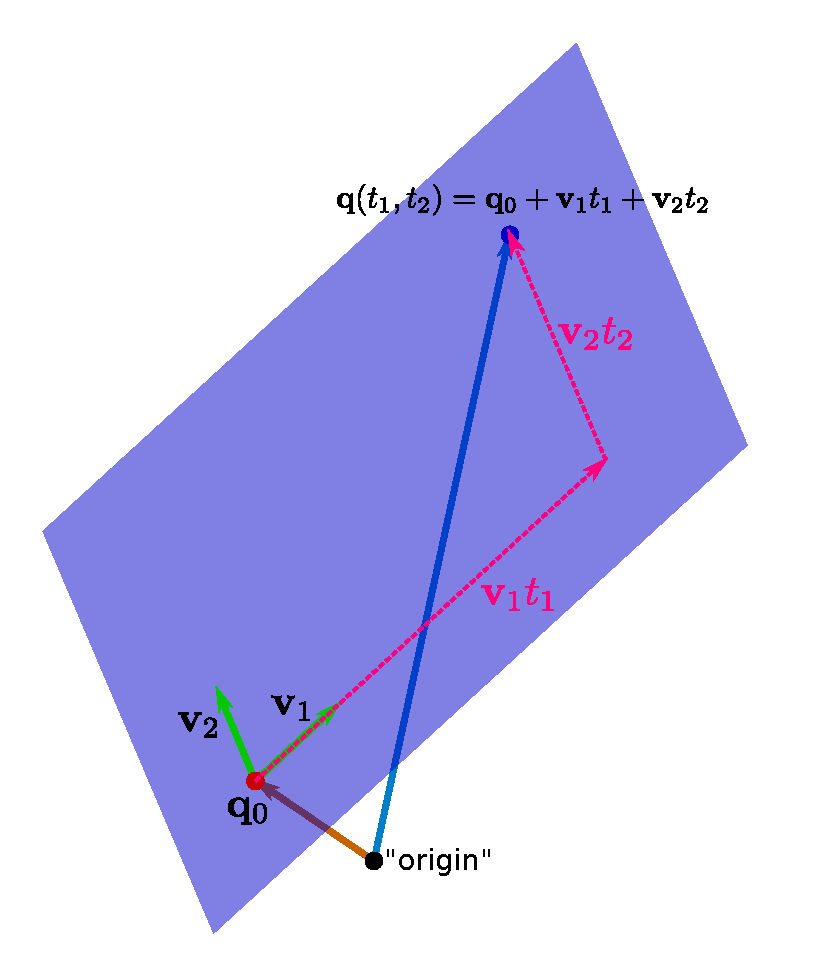
\includegraphics[width = 0.5\textwidth]{vector_equation_plane}
} & \parbox{0.5\textwidth}{
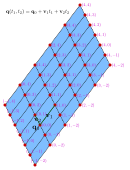
\includegraphics[width = 0.5\textwidth]{plane_parameterization}
}
\end{tabular}

The parametric equations themselves are:
\[\begin{bmatrix} x(t) \\ y(t) \\ z(t) \end{bmatrix} = \begin{bmatrix} x_0 \\ y_0 \\ z_0 \end{bmatrix} + \begin{bmatrix} v_{1x} \\ v_{1y} \\ v_{1z} \end{bmatrix}t_1 + \begin{bmatrix} v_{2x} \\ v_{2y} \\ v_{2z} \end{bmatrix}t_2 = \begin{bmatrix} x_0 + v_{1x} t_1 + v_{2x} t_2 \\ y_0 + v_{1y} t_1 + v_{2y} t_2 \\ z_0 + v_{1z} t_1 + v_{2z} t_2 \end{bmatrix}  
\iff \left\{\begin{array}{c} x(t) = x_0 + v_{1x} t_1 + v_{2x} t_2 \\ y(t) = y_0 + v_{1y} t_1 + v_{2y} t_2 \\ z(t) = z_0 + v_{1z} t_1 + v_{2z} t_2 \end{array}\right.\]

\textbf{Examples:}
\begin{itemize}
%%%%%%%%%%%%%%%%%%%%%%%%%%%
\item Given the points \(T(6, -1, 0)\), \(D(10, -4, -7)\), and \(Q(-1, 0, 2)\) the plane that passes through the points \(T\), \(D\), and \(Q\) must be parallel to \(\overrightarrow{TD} = \begin{bmatrix} 10 - 6 \\ (-4) - (-1) \\ (-7) - 0 \end{bmatrix} = \begin{bmatrix} 4 \\ -3 \\ -7 \end{bmatrix}\) and \(\overrightarrow{TQ} = \begin{bmatrix} (-1) - 6 \\ 0 - (-1) \\ 2 - 0 \end{bmatrix} = \begin{bmatrix} -7 \\ 1 \\ 2 \end{bmatrix}\). One possible vector equation is:
\[\mathbf{q}(t_1, t_2) = \begin{bmatrix} 6 \\ -1 \\ 0 \end{bmatrix} + \begin{bmatrix} 4 \\ -3 \\ -7 \end{bmatrix}t_1 + \begin{bmatrix} -7 \\ 1 \\ 2 \end{bmatrix}t_2\] 
The corresponding set of parametric equations is: 
\[\left\{\begin{array}{c} x(t_1, t_2) = 6 + 4t_1 - 7t_2 \\ y(t_1, t_2) = -1 - 3t_1 + t_2 \\ z(t_1, t_2) = -7t_1 + 2t_2 \end{array}\right.\]
Another set of parametric equations can be derived by observing that the plane passes through the point where \(t_1 = -1\) and \(t_2 = 3\): \(\mathbf{q}(-1, 3) = \begin{bmatrix} -19 \\ 5 \\ 13 \end{bmatrix}\), and is parallel to the vectors \(2\overrightarrow{TD} = \begin{bmatrix} 8 \\ -6 \\ -14 \end{bmatrix}\) and \(\overrightarrow{TD} - 3\overrightarrow{TQ} = \begin{bmatrix}  25 \\ -6 \\ -13 \end{bmatrix}\) Another vector equation {\bf of the same plane} is: 
\[\mathbf{q}(t) = \begin{bmatrix} -19 \\ 5 \\ 13 \end{bmatrix} + \begin{bmatrix} 8 \\ -6 \\ -14 \end{bmatrix}t_1 + \begin{bmatrix} 25 \\ -6 \\ -13 \end{bmatrix}t_2\] 
The corresponding set of parametric equations is: 
\[\left\{\begin{array}{c} x(t_1, t_2) = -19 + 8t_1 + 25t_2 \\ y(t_1, t_2) = 5 - 6t_1 - 6t_2 \\ z(t_1, t_2) = 13 - 14t_1 - 13t_2 \end{array}\right.\]
%%%%%%%%%%%%%%%%%%%%%%%%%%%
\item Given the points \(R(-1, -3, -4)\), \(A(-1, 2, 3)\), and \(N(6, 2, 7)\) the plane that passes through the points \(R\), \(A\), and \(N\) must be parallel to \(\overrightarrow{RA} = \begin{bmatrix} (-1) - (-1) \\ 2 - (-3) \\ 3 - (-4) \end{bmatrix} = \begin{bmatrix} 0 \\ 5 \\ 7 \end{bmatrix}\) and \(\overrightarrow{RN} = \begin{bmatrix} 6 - (-1) \\ 2 - (-3) \\ 7 - (-4) \end{bmatrix} = \begin{bmatrix} 7 \\ 5 \\ 11 \end{bmatrix}\). One possible vector equation is:
\[\mathbf{q}(t_1, t_2) = \begin{bmatrix} -1 \\ -3 \\ -4 \end{bmatrix} + \begin{bmatrix} 0 \\ 5 \\ 7 \end{bmatrix}t_1 + \begin{bmatrix} 7 \\ 5 \\ 11 \end{bmatrix}t_2\] 
The corresponding set of parametric equations is: 
\[\left\{\begin{array}{c} x(t_1, t_2) = -1 + 7t_2 \\ y(t_1, t_2) = -3 + 5t_1 + 5t_2 \\ z(t_1, t_2) = -4 + 7t_1 + 11t_2 \end{array}\right.\]
%%%%%%%%%%%%%%%%%%%%%%%%%%%
\item Given the points \(Y(11, 8, -2)\), \(P(7, 11, -5)\), and \(S(13, 7, -5)\) the plane that passes through the points \(Y\), \(P\), and \(S\) must be parallel to \(\overrightarrow{YP} = \begin{bmatrix} 7 - 11 \\ 11 - 8 \\ (-5) - (-2) \end{bmatrix} = \begin{bmatrix} -4 \\ 3 \\ -3 \end{bmatrix}\) and \(\overrightarrow{YS} = \begin{bmatrix} 13 - 11 \\ 7 - 8 \\ (-5) - (-2) \end{bmatrix} = \begin{bmatrix} 2 \\ -1 \\ -3 \end{bmatrix}\). One possible vector equation is:
\[\mathbf{q}(t_1, t_2) = \begin{bmatrix} 11 \\ 8 \\ -2 \end{bmatrix} + \begin{bmatrix} -4 \\ 3 \\ -3 \end{bmatrix}t_1 + \begin{bmatrix} 2 \\ -1 \\ -3 \end{bmatrix}t_2\] 
The corresponding set of parametric equations is: 
\[\left\{\begin{array}{c} x(t_1, t_2) = 11 - 4t_1 + 2t_2 \\ y(t_1, t_2) = 8 + 3t_1 - t_2 \\ z(t_1, t_2) = -2 - 3t_1 - 3t_2 \end{array}\right.\]
\end{itemize}




\subsection*{Implicit equations for planes}

Any plane has the single implicit equation 
\[ax + by + cz = d\]

\begin{tabular}{cc}
\parbox{0.5\textwidth}{
Given the vector/parametric equations:
\[\mathbf{q}(t_1, t_2) = \mathbf{q}_0 + \mathbf{v}_1 t_1 + \mathbf{v}_2 t_2 \]
which describe a plane, how can an implicit equation be derived? Let \(\mathbf{q}\) be an arbitrary point. The {\bf normal vector} \(\mathbf{n} = \mathbf{v}_1 \times \mathbf{v}_2\) is perpendicular to both \(\mathbf{v}_1\) and \(\mathbf{v}_2\), and is therefore perpendicular to the plane. An arbitrary point \(\mathbf{q}\) is part of the plane if and only if the displacement \(\mathbf{q} - \mathbf{q}_0\) is parallel to the plane, and if therefore perpendicular to \(\mathbf{n}\). This yields the intrinsic equation: 
\begin{align*}
& \mathbf{n} \bullet (\mathbf{q} - \mathbf{q}_0) = 0 \iff \mathbf{n} \bullet \mathbf{q} - \mathbf{n} \bullet \mathbf{q}_0 = 0 \\
& \iff \mathbf{n} \bullet \mathbf{q} = \mathbf{n} \bullet \mathbf{q}_0
\end{align*} 
If \(\mathbf{q}_0 = \begin{bmatrix} x_0 \\ y_0 \\ z_0 \end{bmatrix}\) and \(\mathbf{n} = \begin{bmatrix} a \\ b \\ c \end{bmatrix}\), then the implicit equation is:
\[a x + b y + c z  = a x_0 + b y_0 + c z_0\]
} & \parbox{0.5\textwidth}{
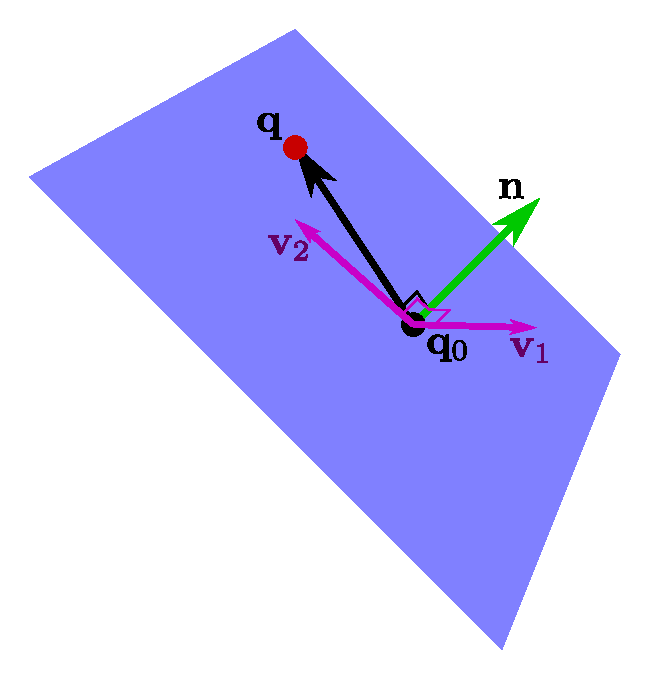
\includegraphics[width = 0.5\textwidth]{implicit_equation_of_the_plane}
}
\end{tabular}

If instead of given the vectors \(\mathbf{q}_0\), \(\mathbf{v}_1\), and \(\mathbf{v}_2\), we were simply given the point \(\mathbf{q}_0\) and \(\mathbf{n} = \begin{bmatrix} a \\ b \\ c \end{bmatrix}\), then the implicit equation is simply \(ax + by + cz = \mathbf{n} \bullet \mathbf{q}_0\).

In reverse, given a plane with the implicit equation \(ax + by + cz = d\), the vector \(\mathbf{n} = \begin{bmatrix} a \\ b \\ c \end{bmatrix}\) is perpendicular to the plane. \(\mathbf{n}\) is referred to as the ``normal vector". The normal vectors can be used to compute the angle between two planes. The angle between two planes is the angle between their normal vectors.

\textbf{Examples:}
\begin{itemize}
%%%%%%%%%%%%%%%%%%%%%%%%%%%
\item Consider the plane \(P\) with the parametric equations: 
\[\left\{\begin{array}{c} x(t_1, t_2) = 6 + 4t_1 - 7t_2 \\ y(t_1, t_2) = -1 - 3t_1 + t_2 \\ z(t_1, t_2) = -7t_1 + 2t_2 \end{array}\right.
\quad\quad\text{the vector equation is:}\quad\quad
\mathbf{q}(t_1, t_2) = \begin{bmatrix} 6 \\ -1 \\ 0 \end{bmatrix} + \begin{bmatrix} 4 \\ -3 \\ -7 \end{bmatrix}t_1 + \begin{bmatrix} -7 \\ 1 \\ 2 \end{bmatrix}t_2\]
An implicit equation for plane \(P\) is sought. \\  
The plane contains the point, \(\mathbf{q}_0 = \begin{bmatrix} 6 \\ -1 \\ 0 \end{bmatrix}\), and is parallel to \(\mathbf{v}_1 = \begin{bmatrix} 4 \\ -3 \\ -7 \end{bmatrix}\) and \(\mathbf{v}_2 = \begin{bmatrix} -7 \\ 1 \\ 2 \end{bmatrix}\). \\
The plane is perpendicular to \(\mathbf{n} = \mathbf{v}_1 \times \mathbf{v}_2 = \begin{bmatrix} (-3)(2) - (-7)(1) \\ (-7)(-7) - (4)(2) \\ (4)(1) - (-3)(-7) \end{bmatrix} = \begin{bmatrix} -6 + 7 \\ 49 - 8 \\ 4 - 21 \end{bmatrix} = \begin{bmatrix} 1 \\ 41 \\ -17 \end{bmatrix}\) \\  
\(\mathbf{n} \bullet \mathbf{q}_0 = (1)(6) + (41)(-1) + (-17)(0) = 6 - 41 + 0 = -35\) \\ 
The implicit equation is:
\[x + 41y - 17z = -35\]
%%%%%%%%%%%%%%%%%%%%%%%%%%%
\item Consider the plane \(P\) with the parametric equations: 
\[\left\{\begin{array}{c} x(t_1, t_2) = -1 + 7t_2 \\ y(t_1, t_2) = -3 + 5t_1 + 5t_2 \\ z(t_1, t_2) = -4 + 7t_1 + 11t_2 \end{array}\right.
\quad\quad\text{the vector equation is:}\quad\quad
\mathbf{q}(t_1, t_2) = \begin{bmatrix} -1 \\ -3 \\ -4 \end{bmatrix} + \begin{bmatrix} 0 \\ 5 \\ 7 \end{bmatrix}t_1 + \begin{bmatrix} 7 \\ 5 \\ 11 \end{bmatrix}t_2\]
An implicit equation for plane \(P\) is sought. \\  
The plane contains the point, \(\mathbf{q}_0 = \begin{bmatrix} -1 \\ -3 \\ -4 \end{bmatrix}\), and is parallel to \(\mathbf{v}_1 = \begin{bmatrix} 0 \\ 5 \\ 7 \end{bmatrix}\) and \(\mathbf{v}_2 = \begin{bmatrix} 7 \\ 5 \\ 11 \end{bmatrix}\). \\
The plane is perpendicular to \(\mathbf{n} = \mathbf{v}_1 \times \mathbf{v}_2 = \begin{bmatrix} (5)(11) - (7)(5) \\ (7)(7) - (0)(11) \\ (0)(5) - (5)(7) \end{bmatrix} = \begin{bmatrix} 55 - 35 \\ 49 - 0 \\ 0 - 35 \end{bmatrix} = \begin{bmatrix} 20 \\ 49 \\ -35 \end{bmatrix}\) \\  
\(\mathbf{n} \bullet \mathbf{q}_0 = (20)(-1) + (49)(-3) + (-35)(-4) = -20 - 147 + 140 = -27\) \\ 
The implicit equation is:
\[20x + 49y - 35z = -27\]
%%%%%%%%%%%%%%%%%%%%%%%%%%%
\item Consider the plane \(P\) with the parametric equations: 
\[\left\{\begin{array}{c} x(t_1, t_2) = 11 - 4t_1 + 2t_2 \\ y(t_1, t_2) = 8 + 3t_1 - t_2 \\ z(t_1, t_2) = -2 - 3t_1 - 3t_2 \end{array}\right.
\quad\quad\text{the vector equation is:}\quad\quad
\mathbf{q}(t_1, t_2) = \begin{bmatrix} 11 \\ 8 \\ -2 \end{bmatrix} + \begin{bmatrix} -4 \\ 3 \\ -3 \end{bmatrix}t_1 + \begin{bmatrix} 2 \\ -1 \\ -3 \end{bmatrix}t_2\]
An implicit equation for plane \(P\) is sought. \\  
The plane contains the point, \(\mathbf{q}_0 = \begin{bmatrix} 11 \\ 8 \\ -2 \end{bmatrix}\), and is parallel to \(\mathbf{v}_1 = \begin{bmatrix} -4 \\ 3 \\ -3 \end{bmatrix}\) and \(\mathbf{v}_2 = \begin{bmatrix} 2 \\ -1 \\ -3 \end{bmatrix}\). \\
The plane is perpendicular to \(\mathbf{n} = \mathbf{v}_1 \times \mathbf{v}_2 = \begin{bmatrix} (3)(-3) - (-3)(-1) \\ (-3)(2) - (-4)(-3) \\ (-4)(-1) - (3)(2) \end{bmatrix} = \begin{bmatrix} -9 - 3 \\ -6 - 12 \\ 4 - 6 \end{bmatrix} = \begin{bmatrix} -12 \\ -18 \\ -2 \end{bmatrix}\) \\  
\(\mathbf{n} \bullet \mathbf{q}_0 = (-12)(11) + (-18)(8) + (-2)(-2) = -132 - 144 + 4 = -272\) \\ 
The implicit equation is:
\[-12x - 18y - 2z = -272\]
%%%%%%%%%%%%%%%%%%%%%%%%%%%
\item Given the point \(Q(7, -1, 2)\) and the line \(L\) defined by the symmetric equations \(\frac{x - 1}{3} = \frac{y + 4}{2} = 5 - z\), an implicit equation of the plane \(P\) that contains point \(Q\) and line \(L\) is sought. \\
To find parametric equations for plane \(P\), two vectors that are parallel to \(P\) must be derived. To start, line \(L\) needs to be placed in parametric form. Let \(t\) denote the common value of \(\frac{x - 1}{3} = \frac{y + 4}{2} = 5 - z\), so \(\frac{x - 1}{3} = t\); \(\frac{y + 4}{2} = t\); and \(5 - z = t\). Solving for each coordinate gives the following parametric equations for line \(L\): 
\[L: \left\{\begin{array}{c} x(t) = 1 + 3t \\ y(t) = -4 + 2t \\ z(t) = 5 - t \end{array}\right.
\quad\quad\text{the vector equation is:}\quad\quad
\mathbf{q}(t) = \begin{bmatrix} 1 \\ -4 \\ 5 \end{bmatrix} + \begin{bmatrix} 3 \\ 2 \\ -1 \end{bmatrix}t\]
Line \(L\) passes through point \(\mathbf{q}_{0L} = \begin{bmatrix} 1 \\ -4 \\ 5 \end{bmatrix}\) and is parallel to the vector \(\mathbf{v}_L = \begin{bmatrix} 3 \\ 2 \\ -1 \end{bmatrix}\). We know that plane \(P\) is parallel to \(\mathbf{v}_L\) and passes through point \(Q(7, -1, 2)\), so let \(\mathbf{q}_0 = \begin{bmatrix} 7 \\ -1 \\ 2 \end{bmatrix}\), and let \(\mathbf{v}_1 = \mathbf{v}_L = \begin{bmatrix} 3 \\ 2 \\ -1 \end{bmatrix}\). The displacement from \(Q\) to any point on \(L\) is also parallel to plane \(P\), so let \(\mathbf{v}_2 = \mathbf{q}_{0L} - \mathbf{q}_0 = \begin{bmatrix} -6 \\ -3 \\ 3 \end{bmatrix}\). A parametric description of plane \(P\) is:
\[\mathbf{q}(t_1, t_2) = \mathbf{q}_0 + t_1\mathbf{v}_1 + t_2\mathbf{v}_2 = \begin{bmatrix} 7 \\ -1 \\ 2 \end{bmatrix} + t_1\begin{bmatrix} 3 \\ 2 \\ -1 \end{bmatrix} + t_2\begin{bmatrix} -6 \\ -3 \\ 3 \end{bmatrix}\]
The plane is perpendicular to \(\mathbf{n} = \mathbf{v}_1 \times \mathbf{v}_2 = \begin{bmatrix} (2)(3) - (-1)(-3) \\ (-1)(-6) - (3)(3) \\ (3)(-3) - (2)(-6) \end{bmatrix} = \begin{bmatrix} 6 - 3 \\ 6 - 9 \\ -9 + 12 \end{bmatrix} = \begin{bmatrix} 3 \\ -3 \\ 3 \end{bmatrix}\) \\
\(\mathbf{n} \bullet \mathbf{q}_0 = (3)(7) + (-3)(-1) + (3)(2) = 21 + 3 + 6 = 30\) \\
The implicit equation is:
\[3x - 3y + 3z = 30\]
which is equivalent to 
\[x - y + z = 10\]
\end{itemize}

\vspace{5mm}

Converting an implicit equation for a plane to a set of parametric equations is simple. Start with the equation \(a x + b y + c z = d\). Solve for one of the coordinates as a function of the other coordinates. Assign to the two ``free" coordinates the parameters \(t_1\) and \(t_2\), and then the solved for coordinate is now a function of \(t_1\) and \(t_2\) as well.

\textbf{Examples:}
\begin{itemize}
%%%%%%%%%%%%%%%%%%%%%%%%%%%
\item Consider the plane \(P\) defined by the equation:
\[3x - 4y + 2z = 6\]
Parametric equations for \(P\) are desired. 
Solving for \(z\) gives:
\[3x - 4y + 2z = 6 \iff 2z = 6 - 3x + 4y \iff z = 3 - \frac{3}{2}x + 2y\]    
Let \(x = t_1\) and \(y = t_2\). \(x\), \(y\), and \(z\) as functions of \(t\) are:
\[\left\{\begin{array}{c}
x(t_1, t_2) = t_1 \\ 
y(t_1, t_2) = t_2 \\ 
z(t_1, t_2) = 3 - \frac{3}{2}t_1 + 2t_2
\end{array}\right.
\quad\quad\text{the vector equation is:}\quad\quad
\mathbf{q}(t_1, t_2) = \begin{bmatrix} 0 \\ 0 \\ 3 \end{bmatrix} + \begin{bmatrix} 1 \\ 0 \\ -\frac{3}{2} \end{bmatrix} t_1 + \begin{bmatrix} 0 \\ 1 \\ 2 \end{bmatrix}t_2\]
%%%%%%%%%%%%%%%%%%%%%%%%%%%
\item Consider the plane \(P\) defined by the equation:
\[3x - 6y = 12\]
Parametric equations for \(P\) are desired. 
Solving for \(z\) gives:
\[3x - 6y = 12 \iff -6y = 12 - 3x \iff y = -2 + \frac{1}{2}x\]    
Let \(x = t_1\) and \(z = t_2\). \(x\), \(y\), and \(z\) as functions of \(t\) are:
\[\left\{\begin{array}{c}
x(t_1, t_2) = t_1 \\ 
y(t_1, t_2) = -2 + \frac{1}{2}t_1 \\ 
z(t_1, t_2) = t_2
\end{array}\right.
\quad\quad\text{the vector equation is:}\quad\quad
\mathbf{q}(t_1, t_2) = \begin{bmatrix} 0 \\ -2 \\ 0 \end{bmatrix} + \begin{bmatrix} 1 \\ \frac{1}{2} \\ 0 \end{bmatrix} t_1 + \begin{bmatrix} 0 \\ 0 \\ 1 \end{bmatrix}t_2\]
%%%%%%%%%%%%%%%%%%%%%%%%%%%
\item Consider the plane \(P\) defined by the equation:
\[4x = 5\]
Parametric equations for \(P\) are desired. 
Solving for \(x\) gives:
\[4x = 5 \iff x = \frac{5}{4}\]    
Let \(y = t_1\) and \(z = t_2\). \(x\), \(y\), and \(z\) as functions of \(t\) are:
\[\left\{\begin{array}{c}
x(t_1, t_2) = \frac{5}{4} \\ 
y(t_1, t_2) = t_1 \\ 
z(t_1, t_2) = t_2
\end{array}\right.
\quad\quad\text{the vector equation is:}\quad\quad
\mathbf{q}(t_1, t_2) = \begin{bmatrix} \frac{5}{4} \\ 0 \\ 0 \end{bmatrix} + \begin{bmatrix} 0 \\ 1 \\ 0 \end{bmatrix} t_1 + \begin{bmatrix} 0 \\ 0 \\ 1 \end{bmatrix}t_2\]
\end{itemize}




\section*{Line-plane intersections}

\begin{tabular}{cc}
\parbox{0.5\textwidth}{
Given a line \(L\) and a plane \(P\), there are \(3\) possible manners as to how the line and plane intersect:
\begin{itemize}
\item In {\bf most cases}, there will be exactly \(1\) intersection. On the right, line \(L_1\) intersects plane \(P\) exactly once. 
\item If the line is embedded in the plane, then the intersection is the line itself and there are infinitely many intersection points. On the right, line \(L_2\) is part of plane \(P\). 
\item If the line is parallel to the plane, but does not touch the plane, then there are 0 intersections. One the right, line \(L_3\) is parallel to plane \(P\) and does not touch plane \(P\).
\end{itemize} 
} & \parbox{0.5\textwidth}{
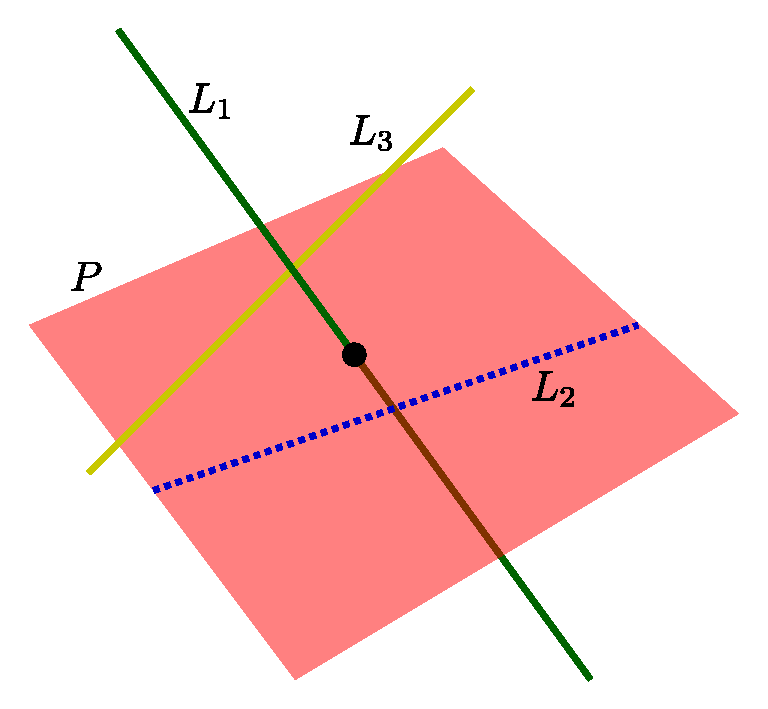
\includegraphics[width = 0.5\textwidth]{line_plane_intersections}
}
\end{tabular}

How can be the intersection be determined? Computing the intersection is easiest when the line is presented using parametric equations, and the plane is presented as a single implicit equation. The expressions for \(x\), \(y\), and \(z\) from the parametric equations are substituted into the plane's equation, and the value of the parameter \(t\) that generates the intersection point is solved for. Once \(t\) has been found, the parametric equations will generate the intersection point \((x, y, z)\). If all possible values of \(t\) solve the equation, the line is contained by the plane. If a contradiction occurs and there is no solution, then no intersection occurs. This is best described by the following examples.

\textbf{Examples:}
\begin{itemize}
%%%%%%%%%%%%%%%%%%%%%%%%%%%%%%%%
\item Let line \(L\) and plane \(P\) have the following descriptions:
\[L : \left\{\begin{array}{c}
x(t) = 1 + 2t \\ 
y(t) = -4 + 3t \\ 
z(t) = -1 - 3t
\end{array}\right. \quad\quad\text{and}\quad\quad 
P : \left\{2x + 2y + z = 35\right.\]
At the intersection point, the point \((x, y, z) = (1 + 2t, -4 + 3t, -1 - 3t)\) generated by the parametric equations must satisfy the equation \(2x + 2y + z = 35\):
\begin{align*}
& 2x + 2y + z = 35 
\iff 2(1 + 2t) + 2(-4 + 3t) + (-1 - 3t) = 35 \\  
& \iff (2 + 4t) + (-8 + 6t) + (-1 - 3t) = 35 
\iff -7 + 7t = 35 \\ 
& \iff 7t = 42 
\iff t = 6  
\end{align*}
The intersection point of \(L\) and \(P\) generated from the parametric equations with \(t = 6\) is:
\[(x, y, z) = (13, 14, -19)\]
%%%%%%%%%%%%%%%%%%%%%%%%%%%%%%%%
\item Let line \(L\) and plane \(P\) have the following descriptions:
\[L : \left\{\begin{array}{c}
x(t) = 6 - t \\ 
y(t) = -2 + 2t \\ 
z(t) = 1 + t
\end{array}\right. \quad\quad\text{and}\quad\quad 
P : \left\{3x + 4y - 5z = 5\right.\]
At the intersection point, the point \((x, y, z) = (6 - t, -2 + 2t, 1 + t)\) generated by the parametric equations must satisfy the equation \(3x + 4y - 5z = 5\):
\begin{align*}
& 3x + 4y - 5z = 5 
\iff 3(6 - t) + 4(-2 + 2t) - 5(1 + t) = 5 \\  
& \iff (18 - 3t) + (-8 + 8t) + (-5 - 5t) = 5 
\iff 5 = 5 
\end{align*}
This equation is always true, so every value of \(t\) generates an intersection point. Line \(L\) is contained by plane \(P\).
%%%%%%%%%%%%%%%%%%%%%%%%%%%%%%%%
\item Let line \(L\) and plane \(P\) have the following descriptions:
\[L : \left\{\begin{array}{c}
x(t) = -1 + 7t \\ 
y(t) = 2 + 3t \\ 
z(t) = 8 - t
\end{array}\right. \quad\quad\text{and}\quad\quad 
P : \left\{2x - 4y + 2z = 1\right.\]
At the intersection point, the point \((x, y, z) = (-1 + 7t, 2 + 3t, 8 - t)\) generated by the parametric equations must satisfy the equation \(2x - 4y + 2z = 1\):
\begin{align*}
& 2x - 4y + 2z = 1 
\iff 2(-1 + 7t) - 4(2 + 3t) + 2(8 - t) = 1 \\  
& \iff (-2 + 14t) + (-8 - 12t) + (16 - 2t) = 1 
\iff 6 = 1 
\end{align*}
This equation is always false, so no value of \(t\) generates an intersection point. Line \(L\) does {\bf not} intersect plane \(P\).
\end{itemize}  




\section*{Plane-plane intersections}

Given two planes \(P_1\) and \(P_2\), there are \(3\) possible manners as to how the planes intersect:
\begin{itemize}
\item In {\bf most cases}, the planes intersect along a line \(L\). In this case, the implicit equations of the planes when put together form the set of implicit equations that describe line \(L\). 
\item If \(P_1 = P_2\), then the intersection is the common plane. 
\item If the planes are parallel but do not touch each other, then there are no intersection points.
\end{itemize} 

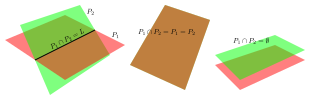
\includegraphics[width = \textwidth]{plane_plane_intersections}

Cases involving planes intersecting along lines were effectively covered when converting the implicit equations of lines to parametric equations. The following examples examine the 2 remaining cases.

\textbf{Examples:}
\begin{itemize}
%%%%%%%%%%%%%%%%%%%%%%%%%%%%%%%%
\item Let planes \(P_1\) and \(P_2\) have the following descriptions:
\[P_1 : \left\{-6x + 10y - 2z = -4\right. \quad\quad\text{and}\quad\quad P_2 : \left\{9x - 15y + 3z = 6\right.\]
What is desired is the set of all \((x,y,z)\) points that satisfy both equations. When solving the system, it is important to determine an ``ordering" for the variables. This ordering will determine which variables are solved for as functions of the other variables. Consider for example the ordering \(x, y, z\). Firstly \(z\) will be solved for in the first equation as a function of the other variables \(x\) and \(y\). 
\[-6x + 10y - 2z = -4 \iff -2z = -4 + 6x - 10y \iff z = 2 - 3x + 5y\]
The expression for \(z\) will then eliminate \(z\) in the second equation. Next \(y\) will be solved for in the second equation as a function of \(x\) alone. 
\begin{align*}
& 9x - 15y + 3z = 6 
\iff 9x - 15y + 3(2 - 3x + 5y) = 6 
\iff 6 = 6 
\end{align*}
This equation is always true, so the only restriction is \(z = 2 - 3x + 5y\). This equation defines a plane, so the intersection is a plane. This means that \(P_1\) and \(P_2\) are the same plane. 
%%%%%%%%%%%%%%%%%%%%%%%%%%%%%%%%
\item Let planes \(P_1\) and \(P_2\) have the following descriptions:
\[P_1 : \left\{21x - 3y + 6z = -3\right. \quad\quad\text{and}\quad\quad P_2 : \left\{-14x + 2y - 4z = 0\right.\]
What is desired is the set of all \((x,y,z)\) points that satisfy both equations. When solving the system, it is important to determine an ``ordering" for the variables. This ordering will determine which variables are solved for as functions of the other variables. Consider for example the ordering \(x, y, z\). Firstly \(z\) will be solved for in the first equation as a function of the other variables \(x\) and \(y\). 
\[21x - 3y + 6z = -3 \iff 6z = -3 - 21x + 3y \iff z = -\frac{1}{2} - \frac{7}{2}x + \frac{1}{2}y\]
The expression for \(z\) will then eliminate \(z\) in the second equation. Next \(y\) will be solved for in the second equation as a function of \(x\) alone. 
\begin{align*}
& -14x + 2y - 4z = 0  
\iff -14x + 2y - 4(-\frac{1}{2} - \frac{7}{2}x + \frac{1}{2}y) = 0  
\iff 2 = 0 
\end{align*}
This equation is always false, so there are no \((x, y, z)\) points that are common to both planes. This means that \(P_1\) and \(P_2\) are parallel, but not the same plane. 
\end{itemize}



\section*{Points and lines}

In {\bf most} cases, given an arbitrary point \(Q\) and a line \(L\), the line \(L\) will {\bf not} pass through point \(Q\). What is often desired instead is the point on line \(L\) that is closest to point \(Q\).  Let the position vector of \(Q\) be \(\mathbf{q}_Q\). Let the vector equation of line \(L\) be:
\[\mathbf{q}(t) = \mathbf{q}_0 + t \mathbf{v}\]

To determine if point \(Q\) lies on line \(L\), one can derive the symmetric equations of line \(L\), and use these equations to decide is \(Q\) lies on \(L\) or not. However, the information that is often desired is not whether or not \(Q\) lies on line \(L\), but how close line \(L\) gets to \(Q\), and what is the closest point on line \(L\) to point \(Q\).

\begin{tabular}{cc}
\parbox{0.5\textwidth}{
If point \(R\) with position vector \(\mathbf{q}_R\) is the point on line \(L\) that is closest to point \(Q\), then the line segment \(RQ\) is perpendicular to line \(L\) as depicted on the right. The closest distance \(d\) between line \(L\) and point \(Q\) is the distance between \(R\) and \(Q\). 
The displacement \(\overrightarrow{RQ} = \mathbf{q}_Q - \mathbf{q}_R\) is the perpendicular component of the displacement \(\mathbf{q}_Q - \mathbf{q}_0\) relative to \(\mathbf{v}\):
\[\mathbf{q}_Q - \mathbf{q}_R = \text{perp}((\mathbf{q}_Q - \mathbf{q}_0)|\mathbf{v})\]
The length of this perpendicular component is:
\[d = \|\text{perp}((\mathbf{q}_Q - \mathbf{q}_0)|\mathbf{v})\| = \frac{\|\mathbf{v} \times (\mathbf{q}_Q - \mathbf{q}_0)\|}{\|\mathbf{v}\|}\] 
} & \parbox{0.5\textwidth}{
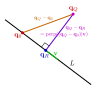
\includegraphics[width = 0.5\textwidth]{point_line_closest_distance}
}
\end{tabular}

If the closest distance \(d\) between point \(Q\) and line \(L\) is all that is needed, then the formula:
\[d = \frac{\|\mathbf{v} \times (\mathbf{q}_Q - \mathbf{q}_0)\|}{\|\mathbf{v}\|}\]
will give that information. However, often the closest point \(R\) itself is also required. As can be easily seen on the right, the displacement \(\mathbf{q}_Q - \mathbf{q}_R\) is perpendicular to \(L\) itself, so \(\mathbf{v} \bullet (\mathbf{q}_Q - \mathbf{q}_R) = 0\). To find \(R\), the value of \(t\) that generates a point \(\mathbf{q}(t)\) on \(L\) where \(\mathbf{v} \bullet (\mathbf{q}_Q - \mathbf{q}(t)) = 0\) needs to be solved for.

\textbf{Example:}
\begin{itemize}
%%%%%%%%%%%%%%%%%%%%%%%%%%%%
\item Consider the point \(Q\) with position vector \(\mathbf{q}_Q = \begin{bmatrix} 2 \\ 3 \\ 1 \end{bmatrix}\) and the line \(L\) with the parametric equations:
\[L: \left\{\begin{array}{c} x(t) = -7 - 2t \\ y(t) = 2 + t \\ z(t) = 2 + t \end{array}\right.\] 
The point \(R\) on line \(L\) that is closest to point \(Q\) and the closest distance \(d\) is desired. 
Line \(L\) passes through \(\mathbf{q}_0 = \begin{bmatrix} -7 \\ 2 \\ 2 \end{bmatrix}\). A displacement parallel to line \(L\) is: \(\mathbf{v} = \begin{bmatrix} -2 \\ 1 \\ 1 \end{bmatrix}\). Next, 
\begin{align*}
\mathbf{v} \bullet (\mathbf{q}_Q - \mathbf{q}(t)) = \begin{bmatrix} -2 \\ 1 \\ 1 \end{bmatrix} \bullet \begin{bmatrix} 9 + 2t \\ 1 - t \\ -1 - t \end{bmatrix} 
= (-18 - 4t) + (1 - t) + (-1 - t) = -18 - 6t
\end{align*}
Now solve for \(t\):
\begin{align*}
\mathbf{v} \bullet (\mathbf{q}_C - \mathbf{q}(t)) = 0 
\iff -18 - 6t = 0 \iff -6t = 18 \iff t = -3
\end{align*}
The closest point \(R\) is:
\[\mathbf{q}(-3) = \begin{bmatrix} -1 \\ -1 \\ -1 \end{bmatrix}\]
The closest distance \(d\) is computed by:
\[\mathbf{q}_Q - \mathbf{q}_0 = \begin{bmatrix} 2 - (-7) \\ 3 - 2 \\ 1 - 2 \end{bmatrix} = \begin{bmatrix} 9 \\ 1 \\ -1 \end{bmatrix}\]
\[\mathbf{v} \times (\mathbf{q}_Q - \mathbf{q}_0) = \begin{bmatrix} -2 \\ 1 \\ 1 \end{bmatrix} \times \begin{bmatrix} 9 \\ 1 \\ -1 \end{bmatrix} 
= \begin{bmatrix} (1)(-1) - (1)(1) \\ (1)(9) - (-2)(-1) \\ (-2)(1) - (1)(9) \end{bmatrix} 
= \begin{bmatrix} -1 - 1 \\ 9 - 2 \\ -2 - 9 \end{bmatrix} = \begin{bmatrix} -2 \\ 7 \\ -11 \end{bmatrix}\]
\[\|\mathbf{v} \times (\mathbf{q}_C - \mathbf{q}_0)\| = \sqrt{4 + 49 + 121} = \sqrt{174}\]
\[\|\mathbf{v}\| = \sqrt{4 + 1 + 1} = \sqrt{6}\]
\[d = \frac{\|\mathbf{v} \times (\mathbf{q}_C - \mathbf{q}_0)\|}{\|\mathbf{v}\|} = \frac{\sqrt{174}}{\sqrt{6}} = \sqrt{29}\]
%%%%%%%%%%%%%%%%%%%%%%%%%%%%
\item Consider the 3 points: \(A(6, -2, 3)\), \(B(4, -1, 2)\), and \(C(5, -4, 6)\). Let line \(L\) pass through points \(A\) and \(B\). The point \(R\) on line \(L\) that is closest to point \(C\) and the closest distance \(d\) is desired. 
Line \(L\) passes through \(\mathbf{q}_0 = \begin{bmatrix} 6 \\ -2 \\ 3 \end{bmatrix}\). A displacement parallel to line \(L\) is: \(\mathbf{v} = \overrightarrow{AB} = \begin{bmatrix} 4 - 6 \\ (-1) - (-2) \\ 2 - 3 \end{bmatrix} = \begin{bmatrix} -2 \\ 1 \\ -1 \end{bmatrix}\). Line \(L\) has vector equation: 
\[\mathbf{q}(t) = \mathbf{q}_0 + t \mathbf{v} = \begin{bmatrix} 6 \\ -2 \\ 3 \end{bmatrix} + t\begin{bmatrix} -2 \\ 1 \\ -1 \end{bmatrix} = \begin{bmatrix} 6 - 2t \\ -2 + t \\ 3 - t \end{bmatrix}\]
The position vector of \(C\) is \(\mathbf{q}_C = \begin{bmatrix} 5 \\ -4 \\ 6 \end{bmatrix}\) so 
\begin{align*}
\mathbf{v} \bullet (\mathbf{q}_C - \mathbf{q}(t)) = \begin{bmatrix} -2 \\ 1 \\ -1 \end{bmatrix} \bullet \begin{bmatrix} -1 + 2t \\ -2 - t \\ 3 + t \end{bmatrix} 
= (2 - 4t) + (-2 - t) + (-3 - t) = -3 - 6t
\end{align*}
Now solve for \(t\):
\begin{align*}
\mathbf{v} \bullet (\mathbf{q}_C - \mathbf{q}(t)) = 0 
\iff -3 - 6t = 0 \iff -6t = 3 \iff t = -\frac{1}{2}
\end{align*}
The closest point \(R\) is:
\[\mathbf{q}(-\frac{1}{2}) = \begin{bmatrix} 7 \\ -5/2 \\ 7/2 \end{bmatrix}\]
The closest distance \(d\) is computed by:
\[\mathbf{q}_C - \mathbf{q}_0 = \begin{bmatrix} 5 - 6 \\ (-4) - (-2) \\ 6 - 3 \end{bmatrix} = \begin{bmatrix} -1 \\ -2 \\ 3 \end{bmatrix}\]
\[\mathbf{v} \times (\mathbf{q}_C - \mathbf{q}_0) = \begin{bmatrix} -2 \\ 1 \\ -1 \end{bmatrix} \times \begin{bmatrix} -1 \\ -2 \\ 3 \end{bmatrix} 
= \begin{bmatrix} (1)(3) - (-1)(-2) \\ (-1)(-1) - (-2)(3) \\ (-2)(-2) - (1)(-1) \end{bmatrix} 
= \begin{bmatrix} 3 - 2 \\ 1 + 6 \\ 4 + 1 \end{bmatrix} = \begin{bmatrix} 1 \\ 7 \\ 5 \end{bmatrix}\]
\[\|\mathbf{v} \times (\mathbf{q}_C - \mathbf{q}_0)\| = \sqrt{1 + 49 + 25} = \sqrt{75} = 5\sqrt{3}\]
\[\|\mathbf{v}\| = \sqrt{4 + 1 + 1} = \sqrt{6}\]
\[d = \frac{\|\mathbf{v} \times (\mathbf{q}_C - \mathbf{q}_0)\|}{\|\mathbf{v}\|} = \frac{5\sqrt{3}}{\sqrt{6}} = \frac{5}{\sqrt{2}}\]
%
%The perpendicular distance \(d\) of point \(C\) from line \(L\) is what is sought. The vector  is parallel to line \(L\). The vector \(\mathbf{v} = \overrightarrow{AC} = \begin{bmatrix} 5 - 6 \\ (-4) - (-2) \\ 6 - 3 \end{bmatrix} = \begin{bmatrix} -1 \\ -2 \\ 3 \end{bmatrix}\) connects a point on line \(L\) to point \(C\). The length of the component of \(\mathbf{v}\) that is perpendicular to line \(L\) is the perpendicular distance \(d\). We first compute:
%\begin{itemize}
%\item[*] \(\|\mathbf{u}\|^2 = \mathbf{u} \bullet \mathbf{u} = (-2)^2 + 1^2 + (-1)^2 = 4 + 1 + 1 = 6\)
%\item[*] \(\|\mathbf{v}\|^2 = \mathbf{v} \bullet \mathbf{v} = (-1)^2 + (-2)^2 + 3^2 = 1 + 4 + 9 = 14\)
%\item[*] \(\mathbf{u} \bullet \mathbf{v} = (-2)(-1) + (1)(-2) + (-1)(3) = 2 - 2 - 3 = -3\)
%\end{itemize} 
%We finally compute:
%\[d = \frac{\sqrt{\|\mathbf{u}\|^2 \|\mathbf{v}\|^2 - (\mathbf{u} \bullet \mathbf{v})^2}}{\|\mathbf{u}\|}
%= \frac{\sqrt{(6)(14) - (-3)^2}}{\sqrt{6}}
%= \frac{\sqrt{84 - 9}}{\sqrt{6}} 
%= \sqrt{\frac{75}{6}}
%= \sqrt{\frac{25}{2}}
%= \frac{5}{\sqrt{2}}\] 
\end{itemize}




\section*{Lines and lines}

In {\bf most} cases, given arbitrary lines \(L_A\) and \(L_B\), these lines will {\bf not} intersect each other. What is often desired instead are the points on line \(L_A\) and line \(L_B\) that are closest to each other. Let the vector equations of lines \(L_A\) and \(L_B\) respectively be:
\[\mathbf{q}_A(t_A) = \mathbf{q}_{0A} + t_A \mathbf{v}_A \quad\quad\text{and}\quad\quad \mathbf{q}_B(t_B) = \mathbf{q}_{0B} + t_B \mathbf{v}_B\]

~\\ \begin{tabular}{cc}
\parbox{0.5\textwidth}{
There are 4 possible relationships two lines may have with each other:
\begin{itemize}
\item The lines intersect at exactly 1 point. 
\item The lines are equivalent. 
\item The lines are not parallel but miss each other. This is referred to as being {\bf skew}. 
\item The lines are parallel but not equivalent. 
\end{itemize}
} & \parbox{0.5\textwidth}{
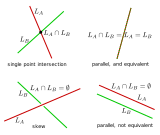
\includegraphics[width = 0.5\textwidth]{line_line_intersections}
}
\end{tabular}

To determine the intersection between two lines (if any exists), both lines need to be presented using parametric equations. The values of the parameters \(t_A\) and \(t_B\) where 
\[\mathbf{q}_A(t_A) = \mathbf{q}_B(t_B)\]
now need to be solved for. 

If there is exactly 1 solution, then the lines intersect at exactly 1 point, the solution being the parameter values that generate the intersection point. If there are infinitely many solutions, then the lines are equivalent. If there are no solutions, then the lines are either parallel without equivalence, or are skew. 

The case of parallel without equivalence and the case of skew are differentiated by checking if the direction vectors \(\mathbf{v}_A\) and \(\mathbf{v}_B\) are parallel or not. If \(\mathbf{v}_A\) and \(\mathbf{v}_B\) are not parallel, then \(L_A\) and \(L_B\) are skew.

\textbf{Examples:}
\begin{itemize}
%%%%%%%%%%%%%%%%%%%%%%%%%%%%%%%%%%
\item Consider lines \(L_A\) and \(L_B\) with the parametric equations:
\[L_A : \left\{\begin{array}{l}
x_A(t_A) = 5 + t_A \\ 
y_A(t_A) = -2 \\ 
z_A(t_A) = 6 + t_A
\end{array}\right.
\quad\quad\text{and}\quad\quad 
L_B : \left\{\begin{array}{l}
x_B(t_B) = t_B \\ 
y_B(t_B) = -17 + 5t_B \\ 
z_B(t_B) = -2 + 2t_B 
\end{array}\right.\]
The parameters \(t_A\) and \(t_B\) that yield the intersection point(s) satisfy:
\[\begin{bmatrix}
5 + t_A \\ 
-2 \\ 
6 + t_A 
\end{bmatrix} = \begin{bmatrix} 
t_B \\ 
-17 + 5t_B \\ 
-2 + 2t_B
\end{bmatrix} \iff 
\left\{\begin{array}{l}
5 + t_A = t_B \\ 
-2 = -17 + 5t_B \\ 
6 + t_A = -2 + 2t_B
\end{array}\right.\]
The first equation yields \(t_B = 5 + t_A\). Eliminating \(t_B\) in the second and third equation yields: 
\[\left\{\begin{array}{l}
-2 = -17 + 5(5 + t_A) \\ 
6 + t_A = -2 + 2(5 + t_A)
\end{array}\right. \iff \left\{\begin{array}{l}
-2 = 8 + 5t_A \\ 
6 + t_A = 8 + 2t_A
\end{array}\right.\]
The second equation yields \(-2 = 8 + 5t_A \iff 5t_A = -10 \iff t_A = -2\). Eliminating \(t_A\) in the third equation yields: 
\[6 + (-2) = 8 + 2(-2) \iff 4 = 4\]
The third equation is always true and can now be ignored. Now evaluating \(t_B\) using the results of the first equation yields: 
\[t_B = 5 + t_A = 3\]
Therefore \(t_A = -2\) and \(t_B = 3\). There is only one solution so \(L_A\) and \(L_B\) intersect exactly once. This intersection point is 
\[(x_A(-2), y_A(-2), z_A(-2)) = (x_B(3), y_B(3), z_B(3)) = (3, -2, 4)\]
%%%%%%%%%%%%%%%%%%%%%%%%%%%%%%%%%%
\item Consider lines \(L_A\) and \(L_B\) with the parametric equations:
\[L_A : \left\{\begin{array}{l}
x_A(t_A) = -2 - 5t_A \\ 
y_A(t_A) = -1 + t_A \\ 
z_A(t_A) = 4 - 3t_A
\end{array}\right.
\quad\quad\text{and}\quad\quad 
L_B : \left\{\begin{array}{l}
x_B(t_B) = -7 - 10t_B \\ 
y_B(t_B) = 2t_B \\ 
z_B(t_B) = 1 - 6t_B 
\end{array}\right.\]
The parameters \(t_A\) and \(t_B\) that yield the intersection point(s) satisfy:
\[\begin{bmatrix}
-2 - 5t_A \\ 
-1 + t_A \\ 
4 - 3t_A 
\end{bmatrix} = \begin{bmatrix} 
-7 - 10t_B \\ 
2t_B \\ 
1 - 6t_B
\end{bmatrix} \iff 
\left\{\begin{array}{l}
-2 - 5t_A = -7 - 10t_B \\ 
-1 + t_A = 2t_B \\ 
4 - 3t_A = 1 - 6t_B
\end{array}\right.\]
The first equation yields \(-2 - 5t_A = -7 - 10t_B \iff -10t_B = 5 - 5t_A \iff t_B = -\frac{1}{2} + \frac{1}{2}t_A\). Eliminating \(t_B\) in the second and third equation yields:
\[\left\{\begin{array}{l}
-1 + t_A = 2(-\frac{1}{2} + \frac{1}{2}t_A) \\ 
4 - 3t_A = 1 - 6(-\frac{1}{2} + \frac{1}{2}t_A)
\end{array}\right. \iff \left\{\begin{array}{l}
-1 + t_A = -1 + t_A \\ 
4 - 3t_A = 4 - 3t_A 
\end{array}\right.\]
Both equations are always true, so the second and third equation can be safely ignored. The only remaining piece of information is an expression for \(t_B\) in terms of \(t_A\) derived from the first equation: \(t_B = -\frac{1}{2} + \frac{1}{2}t_A\). There are infinitely many solutions, so \(L_A = L_B\).
%%%%%%%%%%%%%%%%%%%%%%%%%%%%%%%%%%
\item Consider lines \(L_A\) and \(L_B\) with the parametric equations:
\[L_A : \left\{\begin{array}{l}
x_A(t_A) = -2 - t_A \\ 
y_A(t_A) = 5 + 4t_A \\ 
z_A(t_A) = -1 - t_A
\end{array}\right.
\quad\quad\text{and}\quad\quad 
L_B : \left\{\begin{array}{l}
x_B(t_B) = 6 - 2t_B \\ 
y_B(t_B) = -3t_B \\ 
z_B(t_B) = 4 - t_B 
\end{array}\right.\]
The parameters \(t_A\) and \(t_B\) that yield the intersection point(s) satisfy:
\[\begin{bmatrix}
-2 - t_A \\ 
5 + 4t_A \\ 
-1 - t_A 
\end{bmatrix} = \begin{bmatrix} 
6 - 2t_B \\ 
-3t_B \\ 
4 - t_B
\end{bmatrix} \iff 
\left\{\begin{array}{l}
-2 - t_A = 6 - 2t_B \\ 
5 + 4t_A = -3t_B \\ 
-1 - t_A = 4 - t_B
\end{array}\right.\]
The first equation yields \(-2 - t_A = 6 - 2t_B \iff -2t_B = -8 - t_A \iff t_B = 4 + \frac{1}{2}t_A\). Eliminating \(t_B\) in the second and third equation yields:
\[\left\{\begin{array}{l}
5 + 4t_A = -3(4 + \frac{1}{2}t_A) \\ 
-1 - t_A = 4 - (4 + \frac{1}{2}t_A)
\end{array}\right. \iff \left\{\begin{array}{l}
5 + 4t_A = -12 - \frac{3}{2}t_A \\ 
-1 - t_A = -\frac{1}{2}t_A
\end{array}\right.\]
The second equation yields \(5 + 4t_A = -12 - \frac{3}{2}t_A \iff \frac{11}{2}t_A = -17 \iff t_A = -\frac{34}{11}\). Eliminating \(t_A\) in the third equation yields: 
\[-1 - (-\frac{34}{11}) = -\frac{1}{2}(-\frac{34}{11}) \iff \frac{23}{11} = \frac{17}{11}\]
The third equation is always false, so there are no solutions, and therefore \(L_A\) and \(L_B\) do not intersect. Moreover, the direction vectors are \(\mathbf{v}_A = \begin{bmatrix} -1 \\ 4 \\ -1 \end{bmatrix}\) and \(\mathbf{v}_B = \begin{bmatrix} -2 \\ -3 \\ -1 \end{bmatrix}\). These vectors are not parallel so therefore \(L_A\) and \(L_B\) are skew.
\end{itemize}

\vspace{5mm}

Sometimes, more information than just the intersection point(s) is required. Assume that \(L_A\) and \(L_B\) are not parallel. If points \(\mathbf{q}_{*A}\) and \(\mathbf{q}_{*B}\) are the points on line \(L_A\) and \(L_B\) that are closest, then the displacement \(\mathbf{q}_{*B} - \mathbf{q}_{*A}\) is perpendicular to both lines \(L_A\) and \(L_B\) as depicted below. The closest distance \(d\) between lines \(L_A\) and point \(L_B\) is the length \(R\) and \(\mathbf{q}_{*B} - \mathbf{q}_{*A}\). 
The displacement \(\mathbf{q}_{*B} - \mathbf{q}_{*A}\) is the parallel component of the displacement \(\mathbf{q}_{0B} - \mathbf{q}_{0A}\) relative to \(\mathbf{n} = \mathbf{v}_A \times \mathbf{v}_B\):
\[\mathbf{q}_{*B} - \mathbf{q}_{*A} = \text{proj}((\mathbf{q}_{0B} - \mathbf{q}_{0A})|\mathbf{n})\]
The length of this parallel component is:
\[d = \|\text{proj}((\mathbf{q}_{0B} - \mathbf{q}_{0A})|\mathbf{n})\| = \frac{|\mathbf{n} \bullet (\mathbf{q}_{0B} - \mathbf{q}_{0A})|}{\|\mathbf{n}\|}\] 

If \(d = 0\) then the lines intersect, otherwise they miss each other. %In general, for lines that are not parallel, if \((\mathbf{v}_A \times \mathbf{v}_B) \bullet (\mathbf{q}_{0B} - \mathbf{q}_{0A}) = 0\) if and only if the lines intersect.

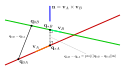
\includegraphics[width = \textwidth]{line_line_closest_distance}

If the closest distance \(d\) between point \(L_1\) and line \(L_2\) is all that is needed, then the formula:
\[d = \frac{|\mathbf{n} \bullet (\mathbf{q}_{0B} - \mathbf{q}_{0A})|}{\|\mathbf{n}\|}\]
will give that information. However, often the closest points \(\mathbf{q}_{*A}\) and \(\mathbf{q}_{*B}\) themselves are also required. As can be easily seen above, the displacement \(\mathbf{q}_{*B} - \mathbf{q}_{*A}\) is perpendicular to both \(L_A\) and \(L_B\), so \(\mathbf{v}_A \bullet (\mathbf{q}_{*B} - \mathbf{q}_{*A}) = 0\) and \(\mathbf{v}_B \bullet (\mathbf{q}_{*B} - \mathbf{q}_{*A}) = 0\). To find \(\mathbf{q}_{*A}\) and \(\mathbf{q}_{*B}\), the values of \(t_A\) and \(t_B\) that respectively generate a point \(\mathbf{q}_A(t_A)\) on \(L_A\) and a point \(\mathbf{q}_B(t_B)\) on \(L_B\) where 
\[\left\{\begin{array}{c}
\mathbf{v}_A \bullet (\mathbf{q}_B(t_B) - \mathbf{q}_A(t_A)) = 0 \\
\mathbf{v}_B \bullet (\mathbf{q}_B(t_B) - \mathbf{q}_A(t_A)) = 0
\end{array}\right.\] 
need to be solved for.

If the lines intersect, then the intersection is the closest point(s). 

\textbf{Examples:}
\begin{itemize}
%%%%%%%%%%%%%%%%%%%%%%%%%%%%
\item Let lines \(L_A\) and \(L_B\) be defined by:
\[L_A : \left\{\begin{array}{c}
x(t) = -2 + 6t \\ 
y(t) = -6 + 3t \\ 
z(t) = 1 
\end{array}\right. \quad\quad\text{and}\quad\quad L_B : \left\{\begin{array}{c}
x(t) = -1 - 2t \\ 
y(t) = -3 - t \\ 
z(t) = 3 + t 
\end{array}\right.\]
The points on \(L_A\) and \(L_B\) that are closest together are what is sought, as well as the minimum distance between these lines.
\[\mathbf{q}_{0A} = \begin{bmatrix} -2 \\ -6 \\ 1 \end{bmatrix} 
\quad\quad\text{and}\quad\quad 
\mathbf{v}_A = \begin{bmatrix} 6 \\ 3 \\ 0 \end{bmatrix}
\quad\quad\text{and}\quad\quad 
\mathbf{q}_{0B} = \begin{bmatrix} -1 \\ -3 \\ 3 \end{bmatrix}
\quad\quad\text{and}\quad\quad
\mathbf{v}_B = \begin{bmatrix} -2 \\ -1 \\ 1 \end{bmatrix}\] 
\[\mathbf{q}_B(t_B) - \mathbf{q}_A(t_A) = \begin{bmatrix}
-1 - 2t_B \\ 
-3 - t_B \\ 
3 + t_B 
\end{bmatrix} - \begin{bmatrix}
-2 + 6t_A \\ 
-6 + 3t_A \\ 
1
\end{bmatrix} = \begin{bmatrix}
1 - 6t_A - 2t_B \\ 
3 - 3t_A - t_B \\ 
2 + t_B
\end{bmatrix}\]
\[\mathbf{v}_A \bullet (\mathbf{q}_B(t_B) - \mathbf{q}_A(t_A)) = (6 - 36t_A - 12t_B) + (9 - 9t_A - 3t_B) + 0 = 15 - 45t_A - 15t_B\]
\[\mathbf{v}_B \bullet (\mathbf{q}_B(t_B) - \mathbf{q}_A(t_A)) = (-2 + 12t_A + 4t_B) + (-3 + 3t_A + t_B) + (2 + t_B) = -3 + 15t_A + 6t_B\]
Now solve for \(t_A\) and \(t_B\): 
\[\left\{\begin{array}{c}
15 - 45t_A - 15t_B = 0 \\ 
-3 + 15t_A + 6t_B = 0
\end{array}\right.\]
Solving the first equation for \(t_B\) gives:
\[15 - 45t_A - 15t_B = 0 \iff -15t_B = -15 + 45t_A \iff t_B = 1 - 3t_A\]
Replacing \(t_B\) in the second equation gives: 
\begin{align*}
& -3 + 15t_A + 6t_B = 0 
\iff -3 + 15t_A + 6(1 - 3t_A) = 0 
\iff -3 + 15t_A + (6 - 18t_A) = 0 \\
& \iff 3 - 3t_A = 0 
\iff -3t_A = -3 
\iff t_A = 1
\end{align*}
Now compute \(t_B = 1 - 3t_A = -2\). \\  
\(t_A = 1\) and \(t_B = -2\). \\  
The point generated on line \(L_A\) is:
\[\mathbf{q}_{*A} = \begin{bmatrix} 4 \\ -3 \\ 1 \end{bmatrix}\]
The point generated on line \(L_B\) is:
\[\mathbf{q}_{*B} = \begin{bmatrix} 3 \\ -1 \\ 1 \end{bmatrix}\] 
The closest distance \(d\) is computed by:
\[\mathbf{q}_{0B} - \mathbf{q}_{0A} = \begin{bmatrix} (-1) - (-2) \\ (-3) - (-6) \\ 3 - 1 \end{bmatrix} = \begin{bmatrix} 1 \\ 3 \\ 2 \end{bmatrix}\]
\[\mathbf{n} = \mathbf{v}_A \times \mathbf{v}_B = \begin{bmatrix} (3)(1) - (0)(-1) \\ (0)(-2) - (6)(1) \\ (6)(-1) - (3)(-2) \end{bmatrix}
 = \begin{bmatrix} 3 - 0 \\ 0 - 6 \\ (-6) + 6 \end{bmatrix} = \begin{bmatrix} 3 \\ -6 \\ 0 \end{bmatrix}\]
\[\mathbf{n} \bullet (\mathbf{q}_{0B} - \mathbf{q}_{0A}) = (3)(1) + (-6)(3) + (0)(2) = 3 - 18 + 0 = -15\]
\[\|\mathbf{n}\| = \sqrt{9 + 36 + 0} = \sqrt{45} = 3\sqrt{5}\]
\[d = \frac{|\mathbf{n} \bullet (\mathbf{q}_{0B} - \mathbf{q}_{0A})|}{\|\mathbf{n}\|} = \frac{|-15|}{3\sqrt{5}} = \sqrt{5}\]
\end{itemize}



\section*{Points and planes}

In {\bf most} cases, given an arbitrary point \(Q\) and a plane \(P\), the plane \(P\) will {\bf not} pass through point \(Q\). What is often desired is the closest distance of point \(Q\) to plane \(P\).  Let the position vector of \(Q\) be \(\mathbf{q}_Q = \begin{bmatrix} x_Q \\ y_Q \\ z_Q \end{bmatrix}\). Let the implicit equation of plane \(P\) be:
\[ax + by + cz = f\]

\begin{tabular}{cc}
\parbox{0.5\textwidth}{
As previously indicated in the description of converting parametric planes to implicit planes, \(\mathbf{n} = \begin{bmatrix} a \\ b \\ c \end{bmatrix}\) is a vector that is perpendicular to plane \(P\). Let \(\mathbf{q}_0 = \begin{bmatrix} x_0 \\ y_0 \\ z_0 \end{bmatrix}\) be an arbitrary point that is on plane \(P\). The implicit equation can be rewritten as 
\[\mathbf{n} \bullet \mathbf{q} = \mathbf{n} \bullet \mathbf{q}_0\]
where \(\mathbf{q} = \begin{bmatrix} x \\ y \\ z \end{bmatrix}\). Therefore \(f = \mathbf{n} \bullet \mathbf{q}_0\). 
The closest distance \(d\) between point \(Q\) and plane \(P\) is the length of the projection of the displacement \(\mathbf{q}_Q - \mathbf{q}_0\) onto \(\mathbf{n}\), as illustrated on the right.  
\begin{align*}
d = & \|\text{proj}((\mathbf{q}_Q - \mathbf{q}_0)|\mathbf{n})\| = \frac{|\mathbf{n} \bullet (\mathbf{q}_Q - \mathbf{q}_0)|}{\|\mathbf{n}\|} \\ 
= & \frac{|\mathbf{n} \bullet \mathbf{q}_Q - \mathbf{n} \bullet \mathbf{q}_0|}{\sqrt{a^2 + b^2 + c^2}}
= \frac{|a x_Q + b y_Q + c z_Q - f|}{\sqrt{a^2 + b^2 + c^2}}
\end{align*}
} & \parbox{0.5\textwidth}{
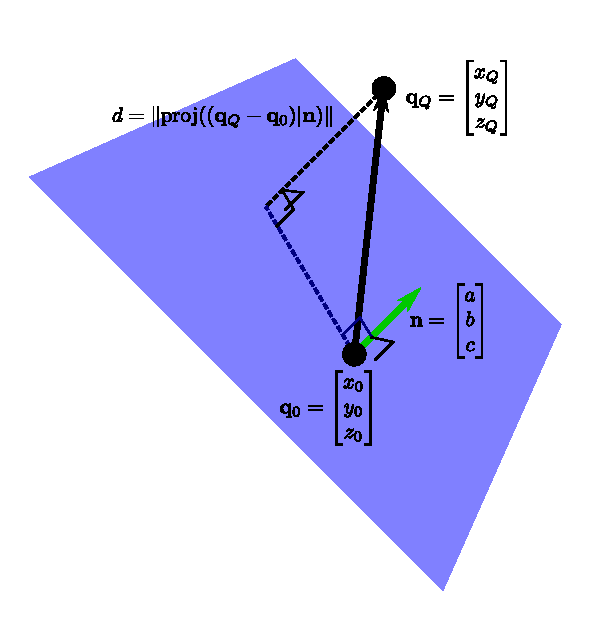
\includegraphics[width = 0.5\textwidth]{point_plane_closest_distance}
}
\end{tabular}
The closest distance between point \(Q\) and plane \(P\) is: 
\[d = \frac{|a x_Q + b y_Q + c z_Q - f|}{\sqrt{a^2 + b^2 + c^2}}\]

\textbf{Examples:}
\begin{itemize}
%%%%%%%%%%%%%%%%%%
\item Consider the point \(Q\) with position vector \(\mathbf{q}_Q = \begin{bmatrix} -5 \\ 0 \\ 1 \end{bmatrix}\) and the plane \(P\) with the implicit equation:
\[P : \left\{-2x + 4y - 3z = 9\right.\] 
The closest distance between point \(Q\) and plane \(P\) is: 
\[d = \frac{|(-2)(-5) + 4(0) - 3(1) - 9|}{\sqrt{4 + 16 + 9}} = \frac{|10 + 0 - 3 - 9|}{\sqrt{29}} = \frac{2}{\sqrt{29}}\]
\end{itemize}


\vspace{5mm}

Now consider two {\bf parallel planes} \(P_A\) and \(P_B\) with the implicit equations:
\[P_A : \left\{a x + b y + c z  = f_A\right. \quad\quad\text{and}\quad\quad P_B : \left\{a x + b y + c z  = f_B\right.\]
Since \(P_A\) and \(P_B\) are parallel, they are both perpendicular to the same vector \(\mathbf{n} = \begin{bmatrix} a \\ b \\ c \end{bmatrix}\), hence why the coefficients of \(x\), \(y\), and \(z\) in the 2 equations are the same. Only the constants on the right hand side are different.  

\begin{tabular}{cc}
\parbox{0.5\textwidth}{
Let \(\mathbf{q}_A = \begin{bmatrix} x_A \\ y_A \\ z_A \end{bmatrix}\) be an arbitrary point from plane \(P_A\) and let \(\mathbf{q}_B = \begin{bmatrix} x_B \\ y_B \\ z_B \end{bmatrix}\) be an arbitrary point from plane \(P_B\). The equations for \(P_A\) and \(P_B\) respectively imply that \(\mathbf{n} \bullet \mathbf{q}_A = f_A\) and that \(\mathbf{n} \bullet \mathbf{q}_B = f_B\). The orthogonal distance between the planes in the length of the projection of the displacement \(\mathbf{q}_B - \mathbf{q}_A\) onto \(\mathbf{n}\), as illustrated on the right. 
\begin{align*}
d = & \|\text{proj}((\mathbf{q}_B - \mathbf{q}_A)|\mathbf{n})\| = \frac{|\mathbf{n} \bullet (\mathbf{q}_B - \mathbf{q}_A)|}{\|\mathbf{n}\|} \\ 
= & \frac{|\mathbf{n} \bullet \mathbf{q}_B - \mathbf{n} \bullet \mathbf{q}_A|}{\sqrt{a^2 + b^2 + c^2}}
= \frac{|f_B - f_A|}{\sqrt{a^2 + b^2 + c^2}}
\end{align*}
} & \parbox{0.5\textwidth}{
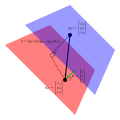
\includegraphics[width = 0.5\textwidth]{plane_plane_distance}
}
\end{tabular}
The orthogonal distance between planes \(P_A\) and \(P_B\) is: 
\[d = \frac{|f_B - f_A|}{\sqrt{a^2 + b^2 + c^2}}\]

\textbf{Examples:}
\begin{itemize}
%%%%%%%%%%%%%%%%%%
\item Consider the two {\bf parallel planes} \(P_A\) and \(P_B\) with the implicit equations:
\[P_A : \left\{2x - 5y + z  = -7\right. \quad\quad\text{and}\quad\quad P_B : \left\{-6x + 15y -3z = -6\right.\]
The equation for \(P_B\) is equivalent to
\[P_B : \left\{2x - 5y + z = 2\right.\] 
The orthogonal distance between planes \(P_A\) and plane \(P_B\) is: 
\[d = \frac{|2 - (-7)|}{\sqrt{4 + 25 + 1}} = \frac{9}{\sqrt{30}}\]
\end{itemize}




\section*{Angles}

When two lines \(L_A : \mathbf{q}_A(t_A) = \mathbf{q}_{0A} + t_A \mathbf{v}_A\) and \(L_B : \mathbf{q}_B(t_B) = \mathbf{q}_{0B} + t_B \mathbf{v}_B\) intersect, the angle between the two lines is the angle between the direction vectors \(\mathbf{v}_A\) and \(\mathbf{v}_B\). 

In a similar vein, the angle between two planes \(a_1 x + b_1 y + c_1 z = d_1\) and \(a_2 x + b_2 y + c_2 z = d_2\) is the angle between the normal vectors \(\mathbf{n}_1 = \begin{bmatrix} a_1 \\ b_1 \\ c_1 \end{bmatrix}\) and \(\mathbf{n}_2 = \begin{bmatrix} a_2 \\ b_2 \\ c_2 \end{bmatrix}\). 

\begin{center}
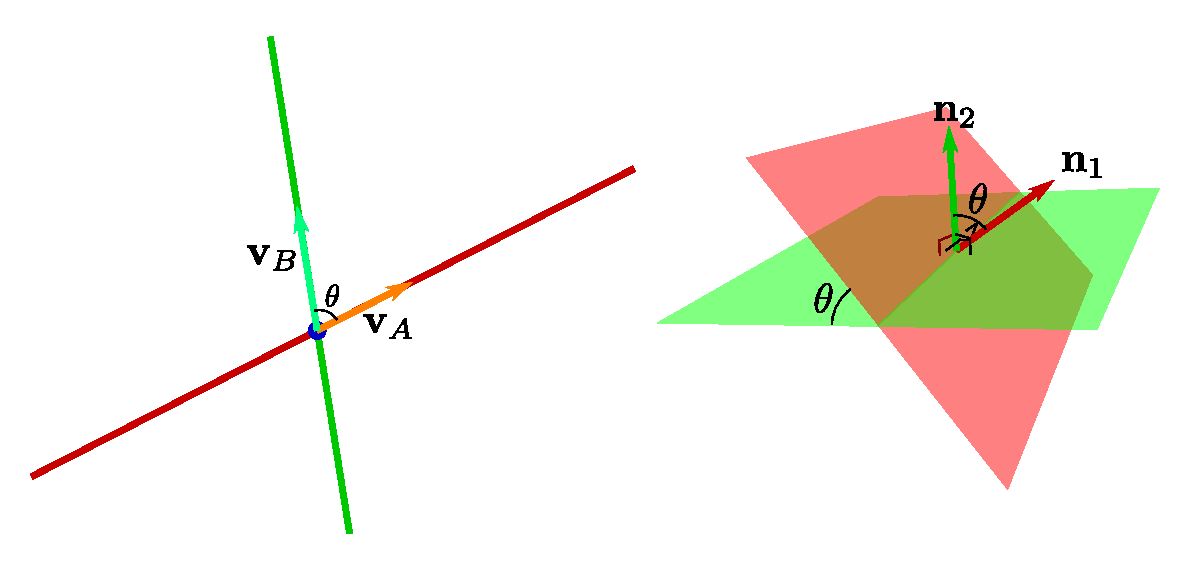
\includegraphics[width = 0.75\textwidth]{line_and_plane_angles} 
\end{center}




\section*{Examples:}

%%%%%%%%%%%%%%%%%%%%%%%%%%%%%%%%%%%%%%%%
%%%%%%%%%%%%%%%%%%%%%%%%%%%%%%%%%%%%%%%%
\subsection*{Example 1:}

Let the points \(P\), \(Q\), and \(R\) be:
\[P(-1, 2, 3) \quad\text{and}\quad Q(2, 1, 2) \quad\text{and}\quad R(5, -1, -1)\] 
\begin{itemize}
%%%%%%%%%%%%%%%%%%%
\item[*] \begin{align*}
\overrightarrow{PQ} = & \begin{bmatrix} 2 - (-1) \\ 1 - 2 \\ 2 - 3 \end{bmatrix} = \begin{bmatrix} 3 \\ -1 \\ -1 \end{bmatrix}
\end{align*}
%%%%%%%%%%%%%%%%%%%
\item[*] The line that passes through points \(P\) and \(Q\) has the vector equation:
\[\begin{bmatrix} x(t) \\ y(t) \\ z(t) \end{bmatrix} = \begin{bmatrix} -1 \\ 2 \\ 3 \end{bmatrix} + t\begin{bmatrix} 3 \\ -1 \\ -1 \end{bmatrix}\] 
and the parametric equations:
\[\left\{\begin{array}{c} 
x(t) = -1 + 3t \\ 
y(t) = 2 - t \\ 
z(t) = 3 - t 
\end{array}\right.\]
To find the symmetric equations, the above parametric equations can be solved to give:
 \[\left\{\begin{array}{ccc} 
x = -1 + 3t & \iff & t = \frac{x+1}{3} \\ 
y = 2 - t & \iff & t = 2 - y \\ 
z = 3 - t & \iff & t = 3 - z
\end{array}\right.\]
Therefore the symmetric equations are:
\[\frac{x+1}{3} = 2 - y = 3 - z\] 
%%%%%%%%%%%%%%%%%%%
\item[*] The distance between points \(P\) and \(Q\) is: 
\[PQ = \left\|\overrightarrow{PQ}\right\| = \sqrt{3^2 + (-1)^2 + (-1)^2} = \sqrt{9 + 1 + 1} = \sqrt{11} \approx 3.31662\]
%%%%%%%%%%%%%%%%%%%
\item[*] \begin{align*}
\overrightarrow{PR} = & \begin{bmatrix} 5 - (-1) \\ (-1) - 2 \\ (-1) - 3 \end{bmatrix} = \begin{bmatrix} 6 \\ -3 \\ -4 \end{bmatrix}
\end{align*}
%%%%%%%%%%%%%%%%%%%
\item[*] The plane that passes through points \(P\), \(Q\), and \(R\) has the vector equation:
\[\begin{bmatrix} x(s, t) \\ y(s, t) \\ z(s, t) \end{bmatrix} = \begin{bmatrix} -1 \\ 2 \\ 3 \end{bmatrix} + s\begin{bmatrix} 3 \\ -1 \\ -1 \end{bmatrix} + t\begin{bmatrix} 6 \\ -3 \\ -4 \end{bmatrix}\] 
and the parametric equations: 
\[\left\{\begin{array}{c} 
x(s, t) = -1 + 3s + 6t \\ 
y(s, t) = 2 - s - 3t \\ 
z(s, t) = 3 - s - 4t 
\end{array}\right.\]
%%%%%%%%%%%%%%%%%%%
\item[*] The plane that passes through points \(P\), \(Q\), and \(R\) is perpendicular to:
\begin{align*}
\mathbf{n} = & \overrightarrow{PQ} \times \overrightarrow{PR} 
= \begin{bmatrix} 3 \\ -1 \\ -1 \end{bmatrix} \times \begin{bmatrix} 6 \\ -3 \\ -4 \end{bmatrix} 
= \begin{bmatrix} 4 - 3 \\ (-6) - (-12) \\ (-9) - (-6) \end{bmatrix} 
= \begin{bmatrix} 1 \\ 6 \\ -3 \end{bmatrix}  
\end{align*}   
%%%%%%%%%%%%%%%%%%%
\item[*] The plane that passes through points \(P\), \(Q\), and \(R\) has the implicit equation:
\begin{align*}
& \mathbf{n} \bullet \left(\begin{bmatrix} x \\ y \\ z \end{bmatrix} - \begin{bmatrix} -1 \\ 2 \\ 3 \end{bmatrix}\right) = 0 
\iff \begin{bmatrix} 1 \\ 6 \\ -3 \end{bmatrix} \bullet \begin{bmatrix} x + 1 \\ y - 2 \\ z - 3 \end{bmatrix} = 0 \\
& \iff (x + 1) + (6y - 12) + (-3z + 9) = 0 \\ 
& \iff x + 6y - 3z - 2 = 0
\end{align*}
%%%%%%%%%%%%%%%%%%%
\item[*] The triangle \(\Delta PQR\) has an area of:   
\begin{align*}
A = & \frac{1}{2}\left\|\overrightarrow{PQ} \times \overrightarrow{PR}\right\|  
= \frac{1}{2}\left\|\begin{bmatrix} 1 \\ 6 \\ -3 \end{bmatrix}\right\| 
= \frac{1}{2}\sqrt{1^2 + 6^2 + (-3)^2} 
= \frac{1}{2}\sqrt{1 + 36 + 9} = \frac{1}{2}\sqrt{46} \approx 3.39116
\end{align*}
\end{itemize}




%%%%%%%%%%%%%%%%%%%%%%%%%%%%%%%%%%%%%%%%
%%%%%%%%%%%%%%%%%%%%%%%%%%%%%%%%%%%%%%%%

\subsection*{Example 2:}

Let the points \(P\), \(Q\), and \(R\) be:
\[P(5, 3, 1) \quad\text{and}\quad Q(6, 5, 2) \quad\text{and}\quad R(-1, 2, 4)\]
\begin{itemize}
%%%%%%%%%%%%%%%%%%%
\item[*] \begin{align*}
\overrightarrow{PQ} = & \begin{bmatrix} 6 - 5 \\ 5 - 3 \\ 2 - 1 \end{bmatrix} = \begin{bmatrix} 1 \\ 2 \\ 1 \end{bmatrix}
\end{align*}
%%%%%%%%%%%%%%%%%%%
\item[*] The line that passes through points \(P\) and \(Q\) has the vector equation:
\[\begin{bmatrix} x(t) \\ y(t) \\ z(t) \end{bmatrix} = \begin{bmatrix} 5 \\ 3 \\ 1 \end{bmatrix} + t\begin{bmatrix} 1 \\ 2 \\ 1 \end{bmatrix}\] 
and the parametric equations:
\[\left\{\begin{array}{c} 
x(t) = 5 + t \\ 
y(t) = 3 + 2t \\ 
z(t) = 1 + t 
\end{array}\right.\]
To find the symmetric equations, the above parametric equations can be solved to give:
 \[\left\{\begin{array}{ccc} 
x = 5 + t & \iff & t = x - 5 \\ 
y = 3 + 2t & \iff & t = \frac{y - 3}{2} \\ 
z = 1 + t & \iff & t = z - 1  
\end{array}\right.\]
Therefore the symmetric equations are:
\[x - 5 = \frac{y - 3}{2} = z - 1\] 
%%%%%%%%%%%%%%%%%%%
\item[*] The distance between points \(P\) and \(Q\) is: 
\[PQ = \left\|\overrightarrow{PQ}\right\| = \sqrt{1^2 + 2^2 + 1^2} = \sqrt{1 + 4 + 1} = \sqrt{6} \approx 2.44949\]
%%%%%%%%%%%%%%%%%%%
\item[*] \begin{align*}
\overrightarrow{PR} = & \begin{bmatrix} (-1) - 5 \\ 2 - 3 \\ 4 - 1 \end{bmatrix} = \begin{bmatrix} -6 \\ -1 \\ 3 \end{bmatrix}
\end{align*}
%%%%%%%%%%%%%%%%%%%
\item[*] The plane that passes through points \(P\), \(Q\), and \(R\) has the vector equation:
\[\begin{bmatrix} x(s, t) \\ y(s, t) \\ z(s, t) \end{bmatrix} = \begin{bmatrix} 5 \\ 3 \\ 1 \end{bmatrix} + s\begin{bmatrix} 1 \\ 2 \\ 1 \end{bmatrix} + t\begin{bmatrix} -6 \\ -1 \\ 3 \end{bmatrix}\] 
and the parametric equations: 
\[\left\{\begin{array}{c} 
x(s, t) = 5 + s - 6t \\ 
y(s, t) = 3 + 2s - t \\ 
z(s, t) = 1 + s + 3t 
\end{array}\right.\]
%%%%%%%%%%%%%%%%%%%
\item[*] The plane that passes through points \(P\), \(Q\), and \(R\) is perpendicular to:
\begin{align*}
\mathbf{n} = & \overrightarrow{PQ} \times \overrightarrow{PR} 
= \begin{bmatrix} 1 \\ 2 \\ 1 \end{bmatrix} \times \begin{bmatrix} -6 \\ -1 \\ 3 \end{bmatrix} 
= \begin{bmatrix} 6 - (-1) \\ (-6) - 3 \\ (-1) - (-12) \end{bmatrix} 
= \begin{bmatrix} 7 \\ -9 \\ 11 \end{bmatrix}  
\end{align*}   
%%%%%%%%%%%%%%%%%%%
\item[*] The plane that passes through points \(P\), \(Q\), and \(R\) has the implicit equation:
\begin{align*}
& \mathbf{n} \bullet \left(\begin{bmatrix} x \\ y \\ z \end{bmatrix} - \begin{bmatrix} 5 \\ 3 \\ 1 \end{bmatrix}\right) = 0 
\iff \begin{bmatrix} 7 \\ -9 \\ 11 \end{bmatrix} \bullet \begin{bmatrix} x - 5 \\ y - 3 \\ z - 1 \end{bmatrix} = 0 \\
& \iff (7x - 35) + (-9y + 27) + (11z - 11) = 0 \\ 
& \iff 7x - 9y + 11z - 19 = 0
\end{align*}   
%%%%%%%%%%%%%%%%%%%
\item[*] The triangle \(\Delta PQR\) has an area of:   
\begin{align*}
A = & \frac{1}{2}\left\|\overrightarrow{PQ} \times \overrightarrow{PR}\right\|  
= \frac{1}{2}\left\|\begin{bmatrix} 7 \\ -9 \\ 11 \end{bmatrix} \right\| 
= \frac{1}{2}\sqrt{7^2 + (-9)^2 + 11^2} 
= \frac{1}{2}\sqrt{49 + 81 + 121} = \frac{1}{2}\sqrt{251} \approx 7.92149
\end{align*}
\end{itemize}

\end{document}






